\documentclass[openany]{book}

\usepackage{generalsnips}
\usepackage{calculussnips}
\usepackage{programmingsnips}
\usepackage[margin = 1in]{geometry}
\usepackage{pdfpages}
\usepackage{amsmath}
\usepackage{amsthm}
\usepackage[utf8]{inputenc}
\usepackage{titlesec}
\usepackage{xpatch}
\usepackage{fancyhdr}
\usepackage{tikz}
\usepackage{hyperref}
\usepackage{minted}
\usepackage{multicol}
\usepackage{float}
\title{Beginning C++ Programming - From Beginner to Beyond}
\date{2020 May 18} % , 12:08PM
\author{David Corzo}

\newcommand{\figs}{./Figs}
\newcommand{\code}{./Code}
\darktheme
\pagestyle{empty}

\begin{document}
\maketitle
\tableofcontents
%%%%%%%%%%%%%%%%%%%%%%%%%%%%%%%%%%%%%%%%%%%%%%%%%%%%%%%%%%%%%%%%%%%%%%%%%%%%%%%%%%%%%%%%%%%%%%%%%%%%%%%%%%%%%%%%%%%%%%%%%%%%%%%%%%%%%%%%%%%%%%

\chapter{Introduction}
\section{What beginners don't know}
\begin{itemize}
    \item Command line basics: 
        \begin{itemize}
            \item Windows, macOS, Linux 
        \end{itemize}
    
    \item Installing python and making it a path environment variable. 
    \item Difference between distributions.
    \item How to google search for answering one's own questions. 
    \item How to run python code. 
    \item Difference between an IDE and python. 
    \item What is syntax highlighting. 
    \item Variables and their purpose. 
\end{itemize}


%----------------------------------------------------------------------------------------

\section{Basic data types}
\begin{center}
    \begin{tabular}{ |l|l| }
        \hline
            Name & Type  \\
        \hline
            Integers & int \\ 
        \hline
            Floating point & float \\ 
        \hline
            Strings & str \\ 
        \hline
            Lists & list \\ 
        \hline
            Dictionaries & dict \\ 
        \hline
            Tuples & tup \\ 
        \hline
            Sets & set \\ 
        \hline
            Booleans & bool \\ 
        \hline
    \end{tabular}
\end{center}


%----------------------------------------------------------------------------------------
\section{Numbers}
\begin{center}
    \begin{tabular}{ |p{5cm}|p{5cm}|p{5cm}| }
        \hline\\[0.25cm]
            Modulo & 20 \% 2 & $\displaystyle 20\times\pmod{2}$  \\[0.45cm]
            \hline
            Powers & 2 ** 2  & $\displaystyle 2^2$  \\[0.45cm]
            \hline
            Floor & 10 // 3  & $\displaystyle \floor{\frac{10}{3} } $  \\[0.45cm]
            \hline
            Grouping & (10 + 3) / 3 & $\displaystyle \frac{10+3}{3} $ \\[0.45cm] 
        \hline
    \end{tabular}
\end{center}

%----------------------------------------------------------------------------------------
\section{Variable names}
Rules: 
\begin{itemize}
    \item No spaces 
    \item Can't use these: \mintinline{python}{;"',<>\()!@#$%^&*~-+|}
    \item Don't use keywords. 
\end{itemize}
\subsection{Dynamic typing}
\begin{itemize}
    \item Python is a dynamically typed language.
    \item This means you can reassign variables to different data types. 
    \item This makes Python very flexible in assigning data types, this is different to other languages that are ``Statically-Typed''.
\end{itemize}
\begin{center}
    \begin{tabular}{ |p{8.5cm}|p{8.5cm}| }
        \hline
            Pros & Cons \\
        \hline
            \begin{itemize}
                \item Easy to work with
                \item Faster development process 
            \end{itemize}
            & 
            \begin{itemize}
                \item May result in bugs for unexpected data types.
                \item You need to be aware of \verb|type()| function to check this. 
            \end{itemize}
            \\ 
        \hline
    \end{tabular}
\end{center}



%----------------------------------------------------------------------------------------
\section{Strings}
\begin{itemize}
    \item In Python ' and " are the same in strings. 
    \item String indexing: used to extract a single character in a string. a[index] 
    \item String slicing: grabs an interval of indexes. a[start:stop:step]
        \begin{itemize}
            \item start: numerical index for the slice start. 
            \item stop index you will go up to but not include. 
            \item step: the size of the jump you take. 
        \end{itemize}
    
    \item Special characters: \verb|\n, \t, \d|
    \item the lenght function: len(a) -$>$ how many elements are in the string. 
\end{itemize}
\subsection{Normal and reverse indexes}
\begin{center}
    \begin{tabular}{ |l|l|l|l|l|l|l|l|l|l|l|l|l| }
        \hline
            H & E & L & L & O &   & W & O & R & L & D & ! \\
            \hline
            0 & 1 & 2 & 3 & 4 & 5 & 6 & 7 & 8 & 9 & 10 & 11 \\ 
            \hline
            0 & -11 & -10 & -9 & -8 & -7 & -6 & -5 & -4 & -3 & -2 & -1 \\ 
        \hline
    \end{tabular}
\end{center}
\subsection{Examples}
\begin{minted}[autogobble]{python}
    # STRING INDEXES AND REVERSE INDEXES
    a = "123456"
    a[1:2] 
    # output: "2" -> Index 1 up to but not including 2
    a[1:3]  
    # output: "23" -> Index 1 up to but not including 3
    a[:3]   
    # output: "123" -> Index 0 (default) up to but not including 3
    a[::]   
    # output: "123456" -> Normal string 
\end{minted}


%----------------------------------------------------------------------------------------
\section{String properties}
\begin{itemize}
    \item Strings are inmutable: 
        \begin{minted}[autogobble]{python}
            name = "david"
            name[0] = "b" 
            # OUTPUT: 
            # Traceback (most recent call last):
            #   File "<stdin>" line 1, in <module>
            # TypeError: 'str' object does not support item assignment
        \end{minted}

        
    
    \item You can concactenate using the + and * signs
        \begin{minted}[autogobble]{python}
            2 + 3 
            # output: 5
            "2" + "3" 
            # output: "23"
            "h" * 10 
            # output: "hhhhhhhhhh" 
        \end{minted}
    
    \item Methods: 
        \begin{itemize}
            \item .upper()
            \item .lower()
            \item .replace()
            \item .split()
        \end{itemize}
\end{itemize}


%----------------------------------------------------------------------------------------
\section{Print formating with strings}
\begin{itemize}
    \item .format() for string interpolation:
        \begin{minted}[autogobble]{python}
            print("this is a string {}".format("inserted"))
            # output: This is a string inserted

            print("The {} {} {}".format("fox","brown","quick"))
            # output:  The fox brown quick 

            print("The {2} {1} {0}".format("fox","brown","quick"))
            # output: The quick brown fox

            print("The {a} {b} {c}".format(a="fox",b="brown",c="quick"))
            # output: The quick brown fox

            result = 100/777
            print(result) 
            # output: 0.1287001287001287
            # Float formatting formula "{value:width.precision f}"
            print("The result was {r:1.3f}".format(r=result))
            # output: The result was 0.129 
        \end{minted}

    \item f-strings for string interpolation: 
        \begin{minted}[autogobble]{python}
            # F-STRING FORMATING
            var = "World"
            print(f"Hello {var}")
            # output: Hello World
        \end{minted}
\end{itemize}

%----------------------------------------------------------------------------------------
\section{Lists}
\begin{itemize}
    \item They suport indexing and slicing.
        \begin{minted}[autogobble]{python}
            my_list = [1,2,3] 
            my_list[1:]
            # output: [2,3]
            another_list = [4,5]
            my_list + another_list 
            # output: [1,2,3,4,5]
        \end{minted}
        
    \item You can also concactenate lists together. 
    \item Lists are mutable. 
\end{itemize}
\subsection{Methods}
\begin{itemize}
    \item .append(\placeholder{something}) -$>$ Appends to the list. 
    \item .sort() -$>$ sorts the iterable alphabetically or numericaly, this is a void, it doen't return anything, don't assign it to anything because it returns None.
        \begin{minted}[autogobble]{python}
            new_list = ['a','e','x','b','c']
            new_list.sort()
            new_list
            # output: ['a','b','c','e','x']
        \end{minted}
        
    \item .pop() $\rightarrow$  eliminates last element and prints it.
        \begin{minted}[autogobble]{python}
            my_list.pop(0) 
            # output: pops element 0.
        \end{minted}
        
    \item .reverse() $\rightarrow$ returns the reverse of the list. 
\end{itemize}

%----------------------------------------------------------------------------------------
\section{Dictionaries}
\begin{itemize}
    \item Doesn't need indexes. Just keys and values. 
    \item Dictionaries are unordered and can't be sorted.
    \item Methods:
        \begin{minted}[autogobble]{python}
            d = {"key1":1,"key2":2}
        \end{minted}
\end{itemize}

\subsection{Methods}
\begin{itemize}
    \item d.keys() $\rightarrow$ returns all the keys in a dictionary.
        \begin{minted}[autogobble]{python}
            d.keys() 
            # output:  dict_keys(['key1','key2'])
        \end{minted}

    \item d.values() $\rightarrow$ returns all the values in a dictionary.
        \begin{minted}[autogobble]{python}
            d.values() 
            # output: dict_values([1,2])
        \end{minted}

\end{itemize}

%----------------------------------------------------------------------------------------
\section{Tuples}
\begin{itemize}
    \item They are immutable lists essentially. 
        \begin{minted}[autogobble]{python}
            t = ('a','a','b')
            t[0] = 'NEW'
            # output: 
            # Traceback (most recent call last):
            #   File "<stdin>", line 1, in <module>
            # TypeError: 'tuple' object does not support item assignment
        \end{minted}
    \item Useful for immutable applications and memory efficiency.
\end{itemize}
\subsection{Methods}
\begin{itemize}
    \item t.count('a') $\rightarrow$ counts the occurrences of 'a' in the tuple. 
    \item t.index('a') $\rightarrow$ returns the index in which the first time 'a' appears. 
\end{itemize}

%----------------------------------------------------------------------------------------
\section{Sets}
\begin{itemize}
    \item Unordered collection of unique elements. 
        \begin{minted}[autogobble]{python}
            my_set = set()
        \end{minted}
    \item There can only be one of each element, no duplicates. 
    \item Useful for duplicate deletion. 
\end{itemize}

\subsection{Methods}
\begin{itemize}
    \item .add() $\rightarrow$ inserts 1 to the set. 
        \begin{minted}[autogobble]{python}
            my_set.add(1) # output: {1}
            my_set.add(2) # output: {1,2}
            my_set.add(2) # output: {1,2} -> doesn't add because that is a duplicate. 
        \end{minted}
\end{itemize}

%----------------------------------------------------------------------------------------
\section{Boolans}
\begin{itemize}
    \item Allows only True, False. 
\end{itemize}

%----------------------------------------------------------------------------------------
\section{Files}
\begin{itemize}
    \item Opening syntax: 
        \begin{minted}[autogobble]{python}
            with open('myfile.txt') as f: 
                contents = f.read()
            # or
            contents = f.read('myfile.txt')
        \end{minted}
\end{itemize}
\subsection{Methods}
\begin{itemize}
    \item .read() $\rightarrow$ returns a string with all the contents of the file. 
    \item .readlines() $\rightarrow$ returns a list with the lines in a file. 
    \item .seek(\placeholder{index}) $\rightarrow$ sets the cursor to the specified index (usually 0).
    \item .truncate() $\rightarrow$ deletes all information in a file. 
    \item .close() $\rightarrow$ closes the file, it's a best practice. 
\end{itemize}
\subsection{Permissions on the with open('myfile.txt') statement }
\begin{itemize}
    \item \mintinline{python}{mode='r'} $\rightarrow$ permissions are enabled to read a file. 
    \item \mintinline{python}{mode='w'} $\rightarrow$ permissions are enabled to write and overwrite to a file, or create a new file. 
    \item \mintinline{python}{mode='r+'} $\rightarrow$ reading and writing permissions.
    \item \mintinline{python}{mode='w+'} $\rightarrow$ writing and reading, overwriting or creating new files. 
    \item \mintinline{python}{mode='a'} $\rightarrow$ appends data to the end of a file, overwriting and writing to a file permissions are enabled. 
\end{itemize}



\chapter{Installation and setup}
\section{Installing C++ Compiler for windows}
\begin{itemize}
    \item Go to: \url{http://mingw-w64.org/doku.php/download/mingw-builds}
    \item Go to: Downloads, find the build, download and run executable.
    \item Set the environment variable:
        \begin{itemize} % [label={$\downarrow$}]
           \item Control panel $\rightarrow$ Edit system environment variables.
           \item Environment variables $\rightarrow$ System $\rightarrow$ Path $\rightarrow$ Edit.
           \item New $\rightarrow$ Browse $\rightarrow$ $<$ go to your instaltion dir $>$ $\rightarrow$ OK.
        \end{itemize}
    
    \item Go to CMD: type \verb|c++ --version| $\rightarrow$ Should print version.
\end{itemize}




\chapter{Curriculum Overview}
\section{Structured Query Language (SQL)}
\begin{itemize}
    \item SQL is a language used for interacting with relational Database Management Systems (RDBMS)
    \item It is kind of like a programming language, it is not strictly a programming language.
    \item You can use SQL to get the RDBMS to do things for you.
        \begin{itemize}
            \item Create, Retrieve, Update and Delete data.
            \item Create and Manage database.
            \item Design and create database tables.
            \item Perform administration tasks (security, user management, import/export, etc)
        \end{itemize}
    
    \item RDBMS do not speak English, they speak SQL.
    \item SQL implementations vary between systems:
        \begin{itemize}
            \item Not all RDBMS' follow the SQL standard to a 'T'.
            \item The concepts are the same but the implementation may vary.
            \item Keep in mind that certain instructions might work on certain RDBMS and not work on others.
        \end{itemize}
    
    \item SQL is actually a hybrid language, it's basically 4 types of languages in one:
        \begin{itemize}
            \item It is a Data Query Language (DQL):
                \begin{itemize}
                    \item Used to query the database for information.
                    \item Get information that is already stored there.
                \end{itemize}
            
            \item Data Definition Language (DDL):
                \begin{itemize}
                    \item Used for defining database schema (A schema is the overall layout of the database such as what columns and rows it will have, what data types are they going to be able to store.)
                \end{itemize}
            
            \item Data Control Language (DCL):
                \begin{itemize}
                    \item Used for controlling access to the data in the database.
                    \item Users and permissions management.
                \end{itemize}
            
            \item Data Manipulation Language (DML):
                \begin{itemize}
                    \item Used for inserting, updating and deleting data from the database.
                \end{itemize}
        \end{itemize}
\end{itemize}

\section{Queries}
\begin{itemize}
    \item A query is a set of instructions given to the RDBMS (written in SQL) that tell the RDBMS what information you want it to retrieve for you.
        \begin{itemize}
            \item There are TONS of data in a database.
            \item Often hidden in a complex schema.
            \item The goal is to only get the data you need.
        \end{itemize}
    
    \item Example: if we want to query the ages and the names of employees in a company that make more than 30000.
        \begin{minted}[autogobble]{sql}
            SELECT employee.name, employee.age
            FROM employee 
            WHERE employee.salary > 30000;
        \end{minted}
\end{itemize}


\chapter{Getting Started}
\section{Intentionality}
\begin{itemize}
    \item The ``aboutness'' of the mind 
    \item Intentionality is the way that the mind is directed at or about the world.
    \item An intentionality state consists of:
        \begin{enumerate}
            \item A propositional content, p
            \item A psychological mode, S
        \end{enumerate}
        it is noted as S(p)
    
    \item Propositional content: 
        \begin{itemize}
            \item Whatever that-clauses contribute to whatever the intentionality is about.
            \item Example:
                \begin{itemize}
                    \item Ralph believes that Jack Sparrow is alive.
                    \item Ralph hopes that Jack Sparrow is alive.
                    \item Ralph desires that Jack Sparrow is alive.
                \end{itemize}
            
            \item This will formally be noted as Ralph: 
                \begin{itemize}
                    \item The first one: Believe(is alive)
                \end{itemize}
        \end{itemize}
    
    \item Psychological mode:
        \begin{itemize}
            \item You can keep the propostional content constant while varying the mode.
            \item There are generic modes.
            \item Some people think tha beliefs and desires can form all teh other modes..
            \item Remember the logical operators and the double negatives.
        \end{itemize}
        \item Conditions of satisfaction:
        \begin{itemize}
            \item The propositional content also determines what will count as it's condition of satisfaction:
                \begin{itemize}
                    \item What makes the belief true? 
                    \item What makes the intentions and desires fulfilled?
                \end{itemize}
            
            \item Propositional content dosnt's have to be text.
            \item Condition of satisfaction is a necesity fulfulled from doing a task.
        \end{itemize}
    
    \item Direction of fit:
        \begin{itemize}
            \item (Water) If I desire water (CoS) when water gets inserted into my mouth that is the condition of satisfaction (Mind)
        \end{itemize}
\end{itemize}



%%%%%%%%%%%%%%%%%%%%%%%%%%%%%%%%%%%%%%%%%%%%%%%%%%%%%%%%%%%%%%%%%%%%%%%%%%%%%%%%%%%%%%%%%%
\section{Sumarry lecture}
\begin{itemize}
    \item We have concepts about objects in propositional content as part of intentional states in the mind.
    \item Concepts, objects are instances of objects.
\end{itemize}



%%%%%%%%%%%%%%%%%%%%%%%%%%%%%%%%%%%%%%%%%%%%%%%%%%%%%%%%%%%%%%%%%%%%%%%%%%%%%%%%%%%%%%%%%%
\section{The network of intentionality and the background}
\begin{itemize}
    \item Intentional states come in a network.
    \item Example: Intend to drive to work, but you can't do that unless you believe you have a job, you have a license, you have teh capacity... 
    \item There form a network not individual units.
    \item Background:   
        \begin{itemize}
            \item Wittgenstein: You woudn't even understand an action with out a background.
            \item We have a hurly-burly that are going on at the same time and only this can give something meaning, this is called background.
            \item If im playing the piano I don't think of how I place fingers but just playing the chords.
        \end{itemize}
    
    \item The ``background'':
        \begin{itemize}
            \item The network is not infinite 
            \item If you follow out the threads and you will find non-intentional states.
            \item You don't belive that your finges can grip the steering wheel you just take that for granted.
            \item This is a very impotant role when we conceptualize anything.
        \end{itemize}
\end{itemize}



%%%%%%%%%%%%%%%%%%%%%%%%%%%%%%%%%%%%%%%%%%%%%%%%%%%%%%%%%%%%%%%%%%%%%%%%%%%%%%%%%%%%%%%%%%
\section{Collective intentionality}
\begin{itemize}
    \item Emerges when we have intentional states about other people's intentionality states.
    \item In coordination with others we create the possibility of collective intentionality.
    \item It emerges as a result of:
        \begin{enumerate}
            \item Multilie people 
            \item Having intentional states andmutual intentional beliefs about 
            \item each other's intentional states.
        \end{enumerate}
    
    \item They have an intenional state of each other's intentional state.
    \item Multiplier effect: 
        \begin{itemize}
            \item Systems exists in out collective intentionality. There are no objective independent systems.
            \item They only exist because I think they exist, you think they exist and I think you think they exist and you think I think they exist.
            \item This is recursive, reciprocity in concepts of one individual with respect to the other.
            \item This is the way we form institutional facts, such examples of these facts is money, money just has value in our minds. 
        \end{itemize}
\end{itemize}


%%%%%%%%%%%%%%%%%%%%%%%%%%%%%%%%%%%%%%%%%%%%%%%%%%%%%%%%%%%%%%%%%%%%%%%%%%%%%%%%%%%%%%%%%%
\section{Sumarry}
\begin{itemize}
    \item We use our concepts about objects and facts in the world as part of the propositional content in intentional states in our minds.
    \item These intentional states come in a network that takes certain background abilities for granted.
\end{itemize}



%%%%%%%%%%%%%%%%%%%%%%%%%%%%%%%%%%%%%%%%%%%%%%%%%%%%%%%%%%%%%%%%%%%%%%%%%%%%%%%%%%%%%%%%%%
\section{Language overview - second corner}
\begin{itemize}
    \item Language: ``The systematic creation maintenance and use of systems of symbols, which dynamically reference concepts and assemble according to structured patterns to communicate meaning''
    \item It's something that is systematic, there are rules, languages also evolves, it's a systems of symbols as well.
    \item Components of languages:
        \begin{enumerate}
            \item Phonology: how words and sentences are pronounced.
            \item Syntax: how words are arranged in sentences.
            \item Semantics: meaning of words and morphems.
            \item Pragmatics: sets general constraints on the use of language.
        \end{enumerate}
    
    \item What do we do with a language? 
        \begin{itemize}
            \item We use language to communicate our intentional states and, as a subset of that, to inform about the world.
        \end{itemize}
\end{itemize}



%%%%%%%%%%%%%%%%%%%%%%%%%%%%%%%%%%%%%%%%%%%%%%%%%%%%%%%%%%%%%%%%%%%%%%%%%%%%%%%%%%%%%%%%%%
\section{Terms and propositions}
\begin{itemize}
    \item Proposition in phylosophy of language:  
        \begin{enumerate}
            \item The ``content'' or ``meaning'' of a meaningful declarative sentence.
            \item The pattern of symbols, marks, or sounds that make up a meaningful declarative sentence.
        \end{enumerate}

    \item A propositions is: 
        \begin{itemize}
            \item A pattern of symbols, a proposition is the pattern of symbols, marks or sounds that make up a meaningful declarative sentence.
        \end{itemize}
    
    \item Symbols (os sign or term etc):
        \begin{itemize}
            \item Link of relationship between the signified and the signifier:
                \begin{itemize}
                    \item The signified is entity in the world or concept in the mind.
                    \item Carl(sign referencing a real person) is a head master(sign refering to a concept ``headmaster'' in the mind).
                \end{itemize}
        \end{itemize}
    
    \item Terms refer to concepts:
        \begin{itemize}
            \item Concepts do not have ``names''
            \item We refer to concepts using signs or terms.
            \item Think of a concept, the concept in the mind doesn't have a name, name the concept agreement or name the concept contract? 
            \item It's a misunderstaning.
            \item This is actually called synonyms and homonyms.
            \item Homonyms and synonyms are common sources for misunderstanding.
        \end{itemize}
\end{itemize}



%%%%%%%%%%%%%%%%%%%%%%%%%%%%%%%%%%%%%%%%%%%%%%%%%%%%%%%%%%%%%%%%%%%%%%%%%%%%%%%%%%%%%%%%%%
\section{Generativity and compositionality}
\begin{itemize}
    \item Features of propositions, propositions have compositionality.
        \begin{itemize}
            \item Compositionality is the framework of rules in which morphemes can be composed, it applies to both syntax and semantics.
            \item The lion ate the apple, or, the apple ate the lion; both have meaning to us.
        \end{itemize}
    
    \item Generativity: is the feature of a language in which it:
        \begin{itemize}
            \item Through recursive syntactical operations (subordinate clauses and conjuntions)
            \item You could produce an infinite number of sentences.
            \item Example: you can append to a sentence more and more compositionality and generativity infinetly.
        \end{itemize}
\end{itemize}

%----------------------------------------------------------------------------------------
\section{Sentence meaning is not enough}
\begin{itemize}
    \item Signs are composed in propositions according to syntactical rules and creates: Sentence meaning.
        \begin{itemize}
            \item Example: can you go to the desk overthere? r// yes i can, I would just use my legs. 
            \item From a sentence meaning it's a correct answer, but clearly the person is asking a favor in the way ``I would like you to go to the desk''
            \item Sentence meaning doesn't transmit intentionality.
            \item This is a computer problem, it's ambiguous to talk to a computer using only sentence meaning, you need to speak literally.
        \end{itemize}
\end{itemize}



%----------------------------------------------------------------------------------------
\section{The king of France is bald}
\begin{itemize}
    \item ``The king of France is bald'' Bertrand Russell.
    \item Natural languages can sometimes be very ambiguous.
    \item If the king of france isn't bald then the negation must be true? this is not always the case.
        \begin{itemize}
            \item \[
              \exists x ( \text{ King of France(x) \&} \forall y(\text{ King of France(y) } \rightarrow y=x) \text{ \& } 
              \text{ Bald }(x)
              )
            \]
            
            \item Or:
                \begin{enumerate}
                    \item There is an $x$ such that $x$ is presently king of France.
                    \item For any $x$ and $y$, if $x$ is presently King of France and $y$ is presently King of France then $x=y$ 
                    \item For every $x$ that is presently King of France, $x$ is bald.
                \end{enumerate}
                \begin{itemize}[label=\#]
                    \item In this case one condition fails, there is no presently a king of France.
                \end{itemize}
        \end{itemize}
\end{itemize}


%----------------------------------------------------------------------------------------
\section{The indeterminancy of translation}
\begin{itemize}
    \item ``The indeterminancy of translation'' Willian Van Oranam Quine.
    \item The rabbit example: ``your out in the bushes, with a native speaker of the language Arunta, a rabbit passes by, he yells 'Gavadai' how could you translate this statement? ''
        \begin{itemize}
            \item Lo food? 
            \item Let's go hunting? 
            \item There will be a storm tonight? 
            \item How do you determine the transation?
            \item This is not about the fact that you don't speak arunta, every child struggles with this, in the bussiness world people speaking the same langueage sometimes are not clear in their comunciations. 
            \item The theory theory ``how do we know that we all have the same concept?''
        \end{itemize}
\end{itemize}



%----------------------------------------------------------------------------------------
\section{Speech acts}
\begin{itemize}
    \item Speech acts are the Uttarances real, intended meaning.
    \item The insufficient sentence meaning, an enourmous amount of background that is presupused when we comunicate. There is always an underlaying background given when we communicate. 
    \newline 
    Example: 
        \begin{itemize}
            \item Let's go out for a drink?
            \item Sorry I can´t, my doctos wond't allow me.
            \item What's the matter with you? 
            \item --------------------------------
            \item Let's go out for a drink?
            \item Sorry,i can't my mother in law won't allow me.
            \item What's the mater with you?
        \end{itemize}
        See the diference? Language is ambigous.
    
    \item We can't spell out all the context, this would make communication imposible, communication is necesarily lacking.
    \item Intentionality's natural extension, intentional states lead to speech acts.
    \item The intentional state ``S'' about a proposition ``p'':
        \[
          \text{ S(p) }
        \]
        Translates to an illocutionary force ``F'' about the same proposition ``p'':
        \[
          \text{ F(p) }
        \]
        Example: ``$\underbrace{\text{ The salt passed to me (p) }}_{\text{ Intentional state }}$ '' $\rightarrow$ ``$\underbrace{\text{ Please hand me the salt! (p) }}_{\text{ Speech act }}$ '' $\rightarrow$ Request (F)
\end{itemize}



%----------------------------------------------------------------------------------------
\section{Meaning through speech acts}
\begin{itemize}
    \item Example: ``$\overbrace{\underbrace{\text{ True is a cat sits on a mat }}_{\text{ Condition of satisfaction }}}^{\text{ Belief (S) }}$'', Intention ``$\underbrace{\text{ This utterance has identical condition of satisfaction as my belief  }}_{\text{ Intention (S) }}$ '' ,the speech act ``$\overbrace{\underbrace{\text{ There is a fluffy mouse catcher on the mat }}_{\text{ (p) }}}^{\text{ Assertion(F) }}$'', given mind to world and a word to fit world.
\end{itemize}



%----------------------------------------------------------------------------------------
\section{Five types of speech acts}
\begin{enumerate}
    \item Asertives:
        \begin{itemize}
            \item Commits a speaker to the truth of the expressed proposition. 
            \item Commits me to the truth given that I said something.
        \end{itemize}
    
    \item Directives:
        \begin{itemize}
            \item Cause the hearer to take a particular action, a request or order.
            \item Example: SALT, NOW! 
        \end{itemize}
    
    \item Commissives:
        \begin{itemize}
            \item That commits a speaker to some future action, a promise.
        \end{itemize}
    
    \item Expressive:
        \begin{itemize}
            \item Used to express the speakers attitudes and emotions towards the proposition.
        \end{itemize}
    
    \item Declarations:
        \begin{itemize}
            \item Change the reality in accordance with the roposition of the declaration, for example declaring someone guilty.
        \end{itemize}
        
\end{enumerate}

They have relation with intentionality:
\begin{itemize}
    \item Asertive $\leftrightarrow $  Belief 
    \item Directive $\leftrightarrow $  Desire 
    \item Commisive $\leftrightarrow $ Intention
    \item Expressive $\leftrightarrow $ Emotive
\end{itemize}


%----------------------------------------------------------------------------------------
\section{The strange thing about declarations}
\begin{itemize}
    \item ``This party starts now'', as Declaration (F): there is no intentional state directly linked to that, I can believe and desire the party has started but it will not start until I perform the declaration.
    \item If you are a judge you can't just judge you have to declare.
    \item Declarations have double direction of fit: Its conditions of satisfaction are fulfilled when:
        \begin{itemize}
            \item The act as such 
            \item Alter the world in the way that 
            \item The world is represented to be altered in propositional content.
        \end{itemize}
        We have double direction of fit.
    
    \item Power of declaration: declarations are one of the most important aspects of language:
        \begin{itemize}
            \item We as humans use this to create our social world.
            \item Declarations are the building blocks of the social world, they are used recursivelly.
            \item Examples: you need to declare it to make it happen.
        \end{itemize}
\end{itemize}



%----------------------------------------------------------------------------------------
\section{Language summary}
\begin{itemize}
    \item We are a reace of humans who have consciousness, intentionality and the capacity of the collective intentionality. We can represent objects and facts that we believe, desire, intent to do, etc. 
    \item  Language has diferent components and on the lowest level, terms are combined into propositions that have sentence meaning.
    \item Language is also the natural extension of the intentionality. Speech acts are utterances real, intended, meaning and is made up os illocunary force and a proposition (statement).
    \item The illocutionary force connects the intentionality with the language usage and corresponding facts and objects in the world.
\end{itemize}


%%%%%%%%%%%%%%%%%%%%%%%%%%%%%%%%%%%%%%%%%%%%%%%%%%%%%%%%%%%%%%%%%%%%%%%%%%%%%%%%%%%%%%%%%%

\section{Metaphysics - introduction}
\begin{itemize}
    \item Metaphysics of the world: objects, properties and relations, facts and truth, functions and social facts.
\end{itemize}


%----------------------------------------------------------------------------------------
\section{Objects}
\begin{itemize}
    \item Objects exists so we need a metaconcept of existance.
    \item Existance - familiar, yet elusive:
        \begin{itemize}
            \item We know how to use the word but have a hard time describing it.
            \item One could be inclined to call only material stuff.
            \item However, that will rule out a lot of the things that we with just a reflection also would call objects. Example: products, agreements, etc. 
            \item A general notion that tends to hold for most situations is ``anything that may be presented to the mind; object of thought''.
        \end{itemize}
    
    \item Concrete objects:
        \begin{itemize}
            \item They only have spatiotemporal properties, they ocupy space and exist for a period of time. Examples: mountains, trees, etc.
            \item Not only spatio-temporal: do human-created material objects exists in the same way as natural objects? Example: upside down woman, upside down table.
            \item Even spaciotemporal objects are always tied to something else.
        \end{itemize}
    
    \item To be or not to be, four different meanings of ``is'', 
        \begin{itemize}
            \item the ``is'' of existance:   
                \begin{itemize}
                    \item ``Socrates is'', $\exists x ( x= \text{ Socrates })$ ''
                \end{itemize}
            
            \item The ``is'' of identity: 
                \begin{itemize}
                    \item ``Hesperus is Phosphorus'' $\text{ Hesperus } = \text{ Phosphorus }$, here we have two words for the same objects.
                \end{itemize}
            
            \item ``The is of predication''
                \begin{itemize}
                    \item ``Socrates is wise'' $\text{ Wise }(\text{ Socrates })$ 
                \end{itemize}
            
            \item ``The ``is'' of general implication'':
                \begin{itemize}
                    \item ``Man is an animal'' $\forall x (\text{ Man }(x) \rightarrow \text{ Animal }(x))$  if $x$ is a man then $x$ is also an animal.
                \end{itemize}
        \end{itemize}
    
    \item Objects of objects: Objects can be composed out of smaller parts, Objects are not always simple, there are objects composed of objects, this is called aggregation. This is called a whole-part relation.
    \item When is an object composed of parts?
        \newline Examples: 
        \begin{itemize}
            \item In contact? Must all parts have to be in contact with each other? is an atom an object? under this definition an atom woudn't be an  object, and that is wrong.
            \item We can say that they must have a force-wise collectively fastened to each other? How much fastened? Example: deck of cards, is it a deck of cards if I spread them around? 
            \item The ``two-woman'': if two people shake and thir fingers get stuck, are they then one object? no, they are still two diferent women.
            \item Maybe there are no composite objects, only mereological simples? indentity crisis? but if there wew only simples, how can human beings with identity exist? we are actually a compositions of a lot of objects.
        \end{itemize}
        A diferent angle: 
        \begin{itemize}
            \item Existence is a. second level feature that applies to concepts, not objects.
            \item That something exists is to say that the concepts have instances.
            \item It's in the concepts, in this way, the existance of composition is dependent on the concepts we have, not a spceific feature of the physical object.
            \item Example: duck or a rabbit? where is the criteria.
        \end{itemize}
\end{itemize}


%----------------------------------------------------------------------------------------
\section{Properties and relations}
\begin{itemize}
    \item Properties: are the 
        \begin{itemize}
            \item attributes or 
            \item qualities or 
            \item features or 
            \item characteristics of 
        \end{itemize}
        things.
    
    \item Phenomena of interest: 
        \begin{itemize}
            \item Properties are typically introduced to help explain or account or phenomena of philosophical interest. 
        \end{itemize}
    
    \item How do we notice properties? when we have a breakdown case: related to phenomenology of Heidegger ``A just perfect hammer for me''
        \begin{itemize}
            \item When the hammer weighs ``just perfect for me '' then we don't hammer and at the same time think ``such a perfect weight for a hammer'' the hammer is just a natural part of the world. I won't think of the hammer if it's perfect for me.
            \item Something stop's us: for some reason we stop and start contemplating the tool, it suddenly for this particular job it's too heavy,
            \item Breakdown case, we contemplate on the hammer and notice that hammers in general could be too light, perfect, too heavy, but they are all for me.
            \item De-worlding: we remove ourselves from the equation and attribute hammers as having weight. If there were no break down case we wouldn't notice the object's properties.
            \item In 99.999\% of the cases we dont notice the properties of an object unless the object doesn't ``do it's job'' or if we are reflecting on the nature of the object.
            \item No breakdown case $\rightarrow$ no property. Example: does money have the propesty weight? in the old times it did, it was a property weight, now there isn't a weight property in today's money.
        \end{itemize}
    
    \item Primary and secondary properties: 
        \begin{itemize}
            \item Primary: properties are objective features of the world: shapes, size, mass, etc. 
            \item Secondary properties are mind-dependent: colors, tests, etc. (intrincic or relative properties)
        \end{itemize}
    
    \item Relations: 
        \begin{itemize}
            \item ``Beind in love is a specific type of property'' love involves multiple types of objects, this is a special property.
            \item Relations are a type of property, relations are properties that exists in multiple things, the property being in love is a two-place relation, there can be multi-place relations as well.
            \item Relations have a single relation: 
                \begin{itemize}
                    \item Romeo $\underbrace{\leftrightarrow }_{\text{ Loves }}$ Juliet
                \end{itemize}
                The objects have roles in the relation or they can be multidimentional.
                \newline Example: 
                \begin{itemize}
                    \item Work well together.
                \end{itemize}
        \end{itemize}
    
    \item Instantiation: ``instantiates'' is a special kind of relation between an object and a propery (concept). 
        \begin{itemize}
            \item Relation between objects and the concept we have in our mind. 
        \end{itemize}
\end{itemize}



%----------------------------------------------------------------------------------------
\section{Facts}
\begin{itemize}
    \item Facts: a situation that the actual world must be in to make a given proposition about the world true: the truth maker.
        \begin{itemize}
            \item At any given situation, the world ob objects with their properties is arranged in a certain way. This we call a fact.
            \item Example: 7 yellow ducks, it is a ``state of affars'' or ``fact''; the proposition ``means'' the fact.
        \end{itemize}
    \item The fact is not just an alone object, the fact obtains if an object excemplifies:
        \begin{enumerate}
            \item at least one property or 
            \item one or mode objects stand in relation 
        \end{enumerate}
        \begin{itemize}
            \item ``A car''is not a fact, ``two pink cars that face each other'' is a fact  they stand in relation and excemplify the properties.
        \end{itemize}
    
    \item The truth-maker and truth bearer: 
        \begin{itemize}
            \item Truth-maker: the fact.
            \item Truth bearer: the actual propoition about the fact. In this relation. 
        \end{itemize}
    
    \item Facts are not true or false: 
        \begin{itemize}
            \item Propositions can be true or false, the truth value is a meta-linguistic property of a proposition. 
            \item A fact in it of itself is not true nor false, or more generically state-of-affairs, can only obtain or fail-to-obtain.
        \end{itemize}
    
    \item Propositions picture simple facts: 
        \begin{itemize}
            \item In the simplest case, the proposition can be thought of as a ``picture'' of the real world fact. The propositional content is the content of the ``picture''.
            \item Counterfactuals are also facts: the negation of some facts. Picture the negation of the fact or the fact with variation, there are endless ways to negate a fact so this is tricky.
        \end{itemize}
    
    \item Facts are any condition that makes a proposition true: 
        \begin{itemize}
            \item Not just a picture.
        \end{itemize}
\end{itemize}



%----------------------------------------------------------------------------------------
\section{Social facts}
\begin{itemize}
    \item All types of objects and properties are involved in facts, not only natural kinds. Example: the money is on the mat, that is a fact.
    \item Objective knowledge: this means that we can have objectively true knowledege about subjective relative phenomena. The statement, proposition can be true, where as tha subjective opinion is isolated. Example: the country is in a resion is a fact based on the subjective fact.
    \item There is no true knowledge at all, because all knowledge is derivated from subjective phenomena, this is called the \textbf{pragmatic truth}.
\end{itemize}


%----------------------------------------------------------------------------------------
\section{Status functions adn institutional facts}
\begin{itemize}
    \item Function: 
        \begin{itemize}
            \item Function is always observer relative, secondary property that is. 
            \item Example: hammer, it's part of a whole, a funtion is defined in a context of others.
            \item Functions are contextualizes explicitly or implicitly in systems.
            \item We assign a function to an object, this function plays a role  in the system.  
        \end{itemize}
    
    \item System has goals: 
        \begin{itemize}
            \item The system strives towars some type of precieved goal, value, purpose or goal, a system. This shoun by the fact that they can fail, or malfunction.
            \item Example: hammer, nails, planks function as a shelter. 
            \item Exists on a background, the whole system axists within an intentional network and preuppose a background. 
            \item Example: I use hammers to drive nails into planks to build a house, which is a shelter. I need shelter because otherwise I would freeze. 
        \end{itemize}
    
    \item No purpose, goal os value, no function: true also for bio-physical function. 
        \begin{itemize}
            \item This is true for all systems.
            \item Biological functions are assigner in respect of some higher imposed value.
            \item The function server a role in the explanation of a theory.
            \item The functions are no intrinsic: We impose them on organs to explein them, if you cahnge the value to destruction from survical, then the organs are malfunctioning, the system always strive to accomplish a higher goal or purpose.
        \end{itemize}
    
    \item Status functions: A special type of agentive function is the status function. We use the declaration speech act to create a function. Example: ``this hereby counts as money in this room'' if everyone accepts this declaration then that piece of paper is money in that room. 
     \newline  We impose functions on objects using declaration of the format:
        \[
          X \; \text{ counts as }\, Y \; \text{ in } \; C
        \]
        
    \item Recursion does the rest for us: 
        \begin{itemize}
            \item This is the way we create social reality.
            \item We declare status functions with the format and then we use recursion to construct the social reality.
        \end{itemize}
    
    \item Steps for status functions:
        \begin{enumerate}
            \item Declare a system 
                \begin{itemize}
                    \item Example: there is hereby a concept called money which the central bank is our state is allowed to issue. Declaration (F).
                \end{itemize}
            \item Recognize and accept: 
                \begin{itemize}
                    \item Everyone accepts the intitution and the money concept.
                \end{itemize}
            
            \item Assign a function to agents: 
                \begin{itemize}
                    \item Who does what.
                \end{itemize}
            
            \item Recognize and accept the declaration of powers: 
                \begin{itemize}
                    \item We know the concept and assign status functions to the concept and object.
                \end{itemize}
            
            \item Declare intitutional facts:
                \begin{itemize}
                    \item We trust and know the social facts of intitutions.
                    \item Recursion
                \end{itemize}
        \end{enumerate}
    
    \item Functions in ``thin air'':
        \begin{itemize}
            \item They don't need for an object at all, these function are called be Searle ``free-standing Y terms'', there is no X in the statement.
            \item You can have a status function without the X.
            \item The normal status function has the power to issuea declaration, example: ``thereby counts as a corporation (declaration F)'' Corporation is Y, the word corporation is Y, a corporation exists from the declaration, and is sometimes independent of X.
            \item We can't do this without language, we can't just think and make it so, a declaration is requiered.
            \item Language is super important.
        \end{itemize}
    
    \item With: 
        \begin{enumerate}
            \item Collective intentionality.
            \item Declare speech acts and
            \item Recursion 
        \end{enumerate}
        We create our social world:
        \begin{itemize}
            \item This realli exists in our collective minds, somethings don't exist out of the social collective mind.
        \end{itemize}
    
        
    \item Things can exist in diferent forms:
        \begin{center}
           \begin{tabular}{ | p{5cm} | p{5cm} | p{5cm} | }
               \hline
                   Exists independently to us & Exists since we use and treat as such & Exists since we have jointly declared them to do so     \\
               \hline
                    \begin{itemize}
                        \item Human
                        \item Being 
                        \item Bacteria 
                        \item Sun 
                        \item Tree 
                        \item Mountain 
                        \item Earth 
                        \item River 
                    \end{itemize}
                    & 
                    \begin{itemize}
                        \item Hammer 
                        \item Table 
                        \item Computer 
                        \item Screwdriver 
                        \item Fork 
                        \item Engine 
                        \item Thermometer
                    \end{itemize}
                    & 
                    \begin{itemize}
                        \item University degree 
                        \item Birthday party 
                        \item President 
                        \item Money 
                        \item Loan 
                        \item Insurance 
                    \end{itemize} 
                    \\ 
               \hline
           \end{tabular}
        \end{center}
        \begin{itemize}
            \item We use language to create social reality.
        \end{itemize}
\end{itemize}


%----------------------------------------------------------------------------------------
\section{The triangle in new light - Summary}
\begin{enumerate}
    \item We take for granted that there are concrete objects and state of affairs that exists.
    \item We have concepts about these objects 
    \item We form intentional states based on the concepts 
    \item We use language signs that represent the objects and concepts.
    \item We make declarations of new concepts and assignments of these.
    \item Those status functions are collectively rectognized and accepted
    \item We apply the new concept and thus we create new abstract objects in the world.
    \item Repeat and repeat.
\end{enumerate}
This is done very implicitly, the objective is to grab those facts and objects and make them explicit.

%----------------------------------------------------------------------------------------
\section{Resources}
\begin{itemize}
    \item Making the social world 
\end{itemize}


\chapter{Structure of a C++ program}
\section{Introduction to linked lists}
\begin{itemize}
    \item Linked lists resolve the problems commonly encountered with arrays, that is the fact that arrays have to be declared of a fixed size and can't really be dynamically grown without fragmenting memory is a problem we can resolve using a linked list data structure.
    \item The draw backs of arrays are actually removed with linked lists at the cost of the benefits of having an array.
\end{itemize}

\subsection{What is wrong with arrays?}
\begin{itemize}
    \item The first issue with array is the size of the array needs to be declared. Using realloc() will not really resolve this because it will copy all the elements of the array in to a bigger memory location, this causes poor performance and fragmentation. 
    \item Once allocated with a size it is a hazard to change the size of the array in runtime.
    \item Another issue is performing the insertion and deletion operation at any point between the first and the last index of the existing elements. An example can clarify this problem.
        \begin{center}
    \begin{bytefield}{10}
        \bitboxes{1}{
            {9} {3} {7} {5} {8} {7} {9} {1} {0} {2}
            } \\ 
        \bitheader{0-9} 
    \end{bytefield}
    \begin{itemize}
        \item If we wanted to delete 5 we need to delete and shift the rest of the array to the left.
    \end{itemize}
    \begin{bytefield}{10}
        \bitboxes{1}{
            {9} {3} {7} {} {8} {7} {9} {1} {0} {2}
            } \\ 
        \bitheader{0-9} 
    \end{bytefield}
    \begin{bytefield}{10}
        \bitboxes{1}{
            {9} {3} {7} {8} {7} {9} {1} {0} {2} {}
            } \\ 
        \bitheader{0-9} 
    \end{bytefield}
    \begin{itemize}
        \item This takes time and impacts performance for large arrays.
        \item This can happen also for insertion. Let's consider we need to insert 5 back in to the array.
        \item First move everything to the right. And then insert the 5.
    \end{itemize}
    \begin{bytefield}{10}
        \bitboxes{1}{
            {9} {3} {7} {} {8} {7} {9} {1} {0} {2} 
            } \\ 
        \bitheader{0-9} 
    \end{bytefield}
    \begin{bytefield}{10}
        \bitboxes{1}{
            {9} {3} {7} {5} {8} {7} {9} {1} {0} {2} 
            } \\ 
        \bitheader{0-9} 
    \end{bytefield}
    \begin{itemize}
        \item See you need to move all the $(n-1)$  elements for every insertion and deletion.
        \item For this we need a linked list rather than an array.
    \end{itemize}
\end{center}

    
    \item Adding a new element or deleting an existing element is independent to the number of elements in the linked list, no shifting kind of activities like arrays are required. 
\end{itemize}


%----------------------------------------------------------------------------------------
\section{Definition of linked list, conception of node, understanding basic principles}
\begin{itemize}
    \item Linked lists are dynamic, created on ``as and when required basis''.
    \item We don't need to specify the size in a linked list.
    \item Elements in a linked list are discrete, not contiguous like arrays.
\end{itemize}

\subsection{Example for storing a set of integers}
\begin{itemize}
    \item Lets declared a structure or node in this case containing members int and pointer. The int is to store the data and the pointer is to store the address of the next node. 
\end{itemize}
\begin{figure}[H]
    \centering
    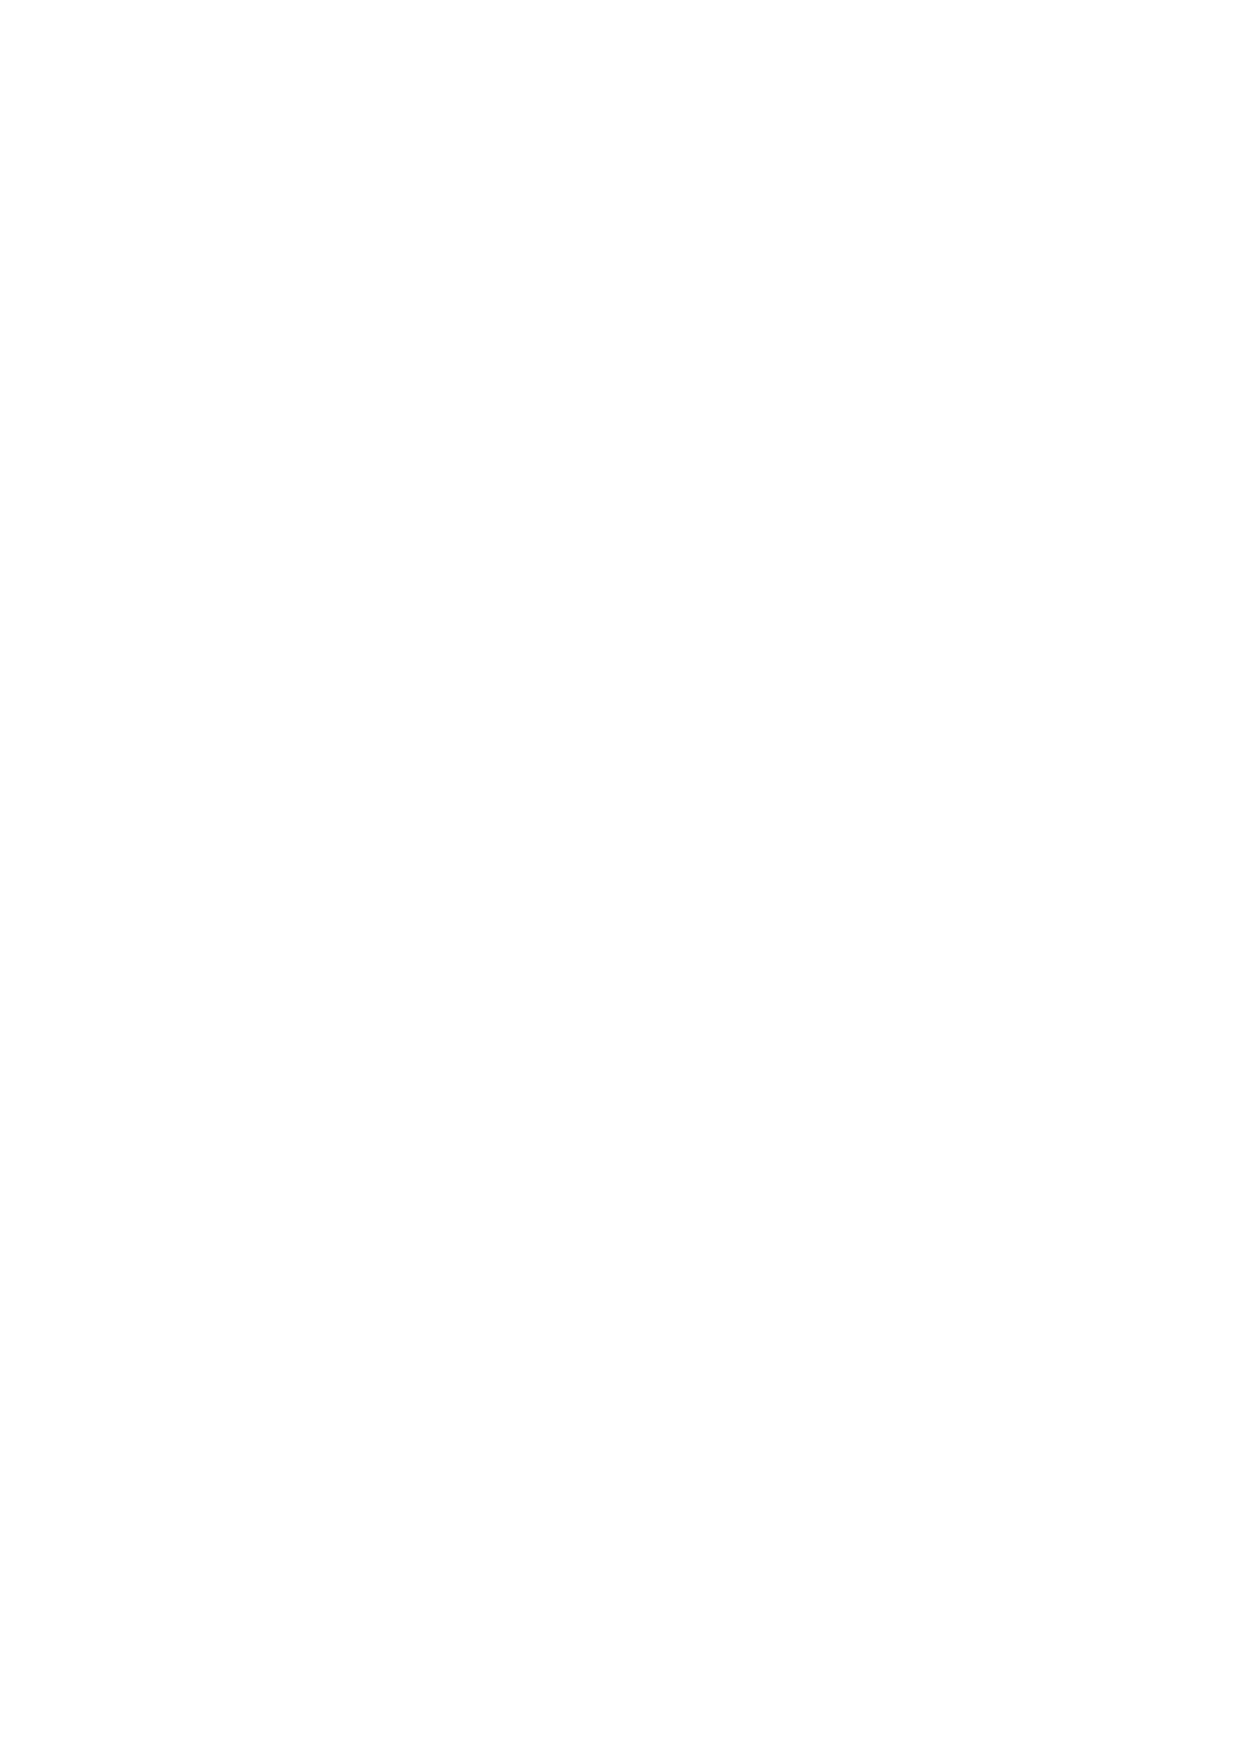
\includegraphics[]{\figs/introll} 
\end{figure}


%----------------------------------------------------------------------------------------
\section{Categories of linked lists - singly, doubly and circular linked list}

\subsection{Singly linked lists}
\begin{itemize}
    \item Consists of nodes containing a data and pointer member, each pointer points to the next node and the tail is recognized when a null pointer is encountered. 
\end{itemize}
\begin{figure}[H]
    \centering
    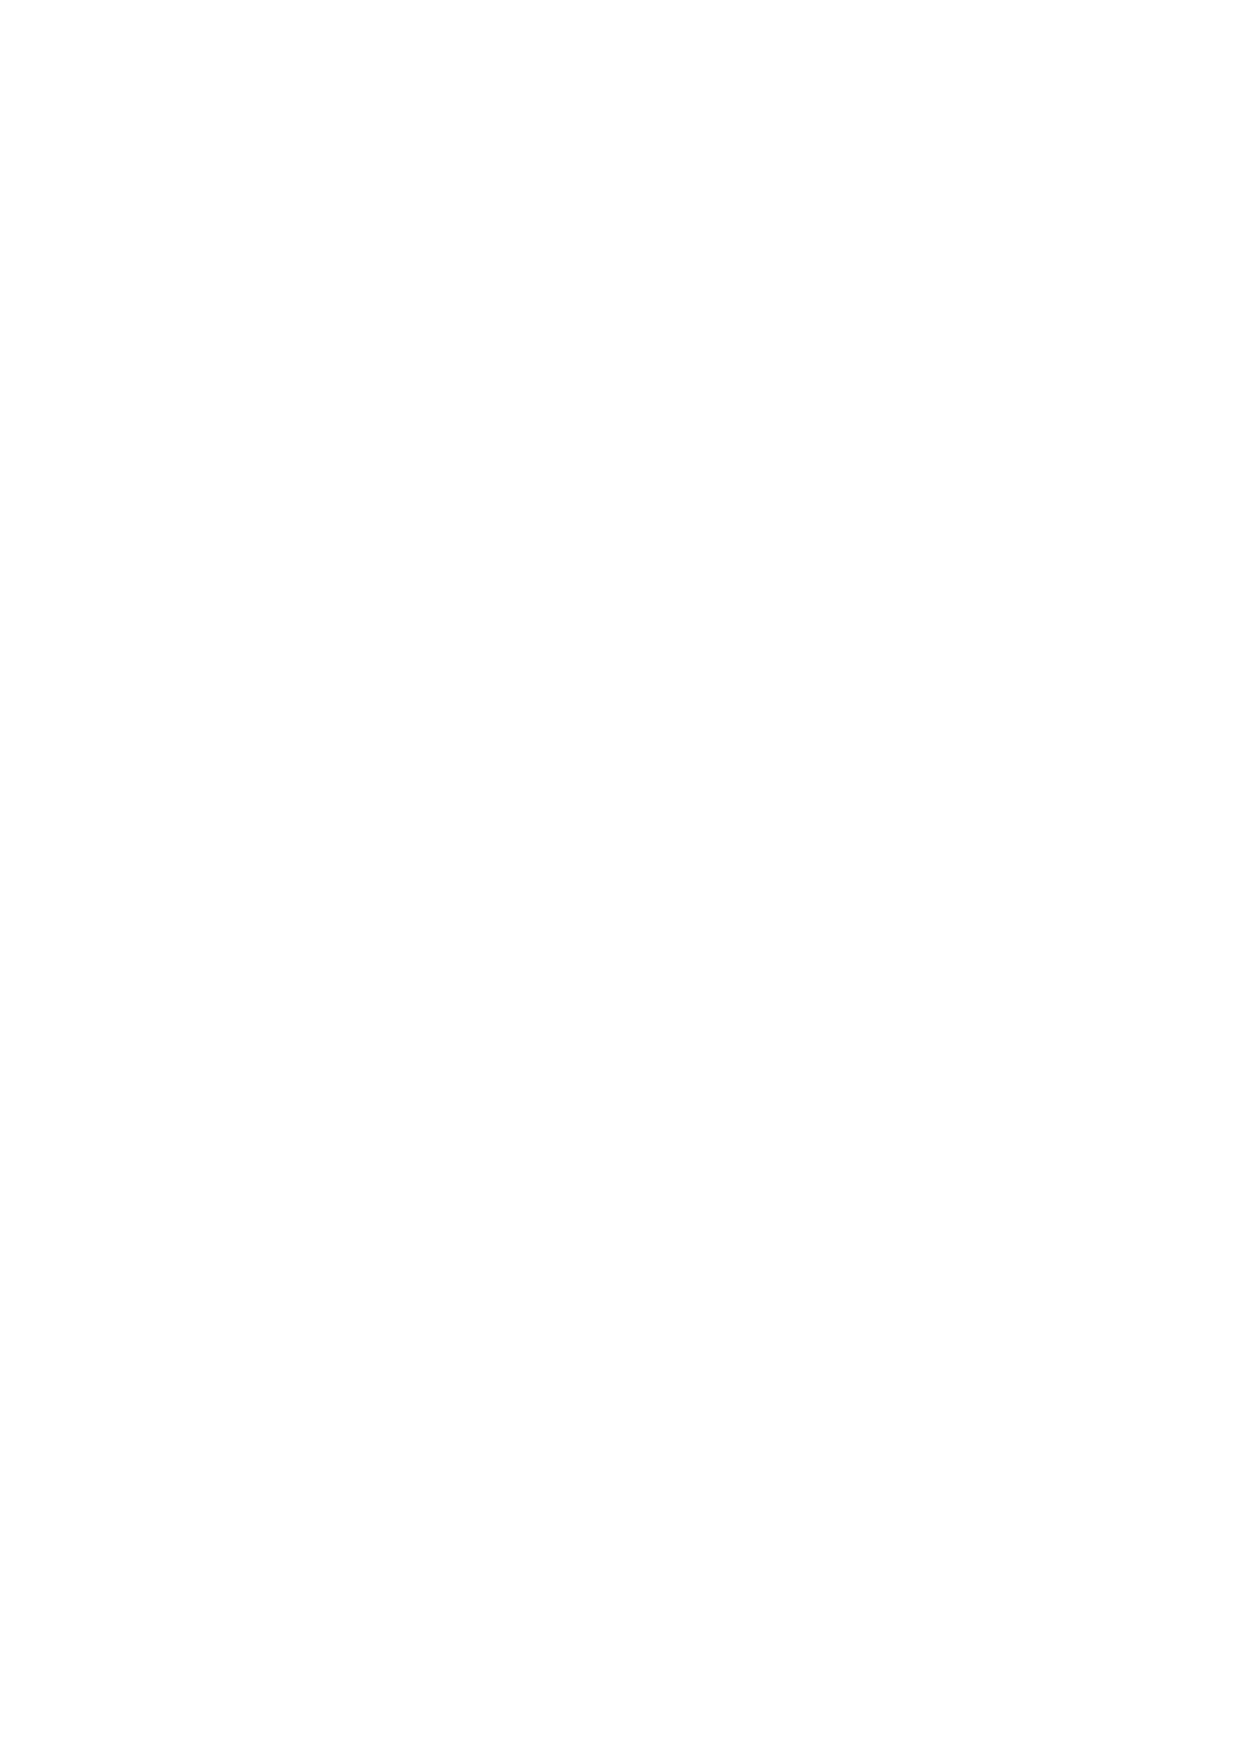
\includegraphics[]{\figs/introsll} 
\end{figure}

\subsection{Circular linked list}
\begin{itemize}
    \item In circular linked list there is no head, there is only a tail pointer, the tail pointer points to the last node's address.
    \item The terminal node does not point to null, it points to the first member of the linked list.
    \item This is based on the circular queue model.
\end{itemize}
\begin{figure}[H]
    \centering
    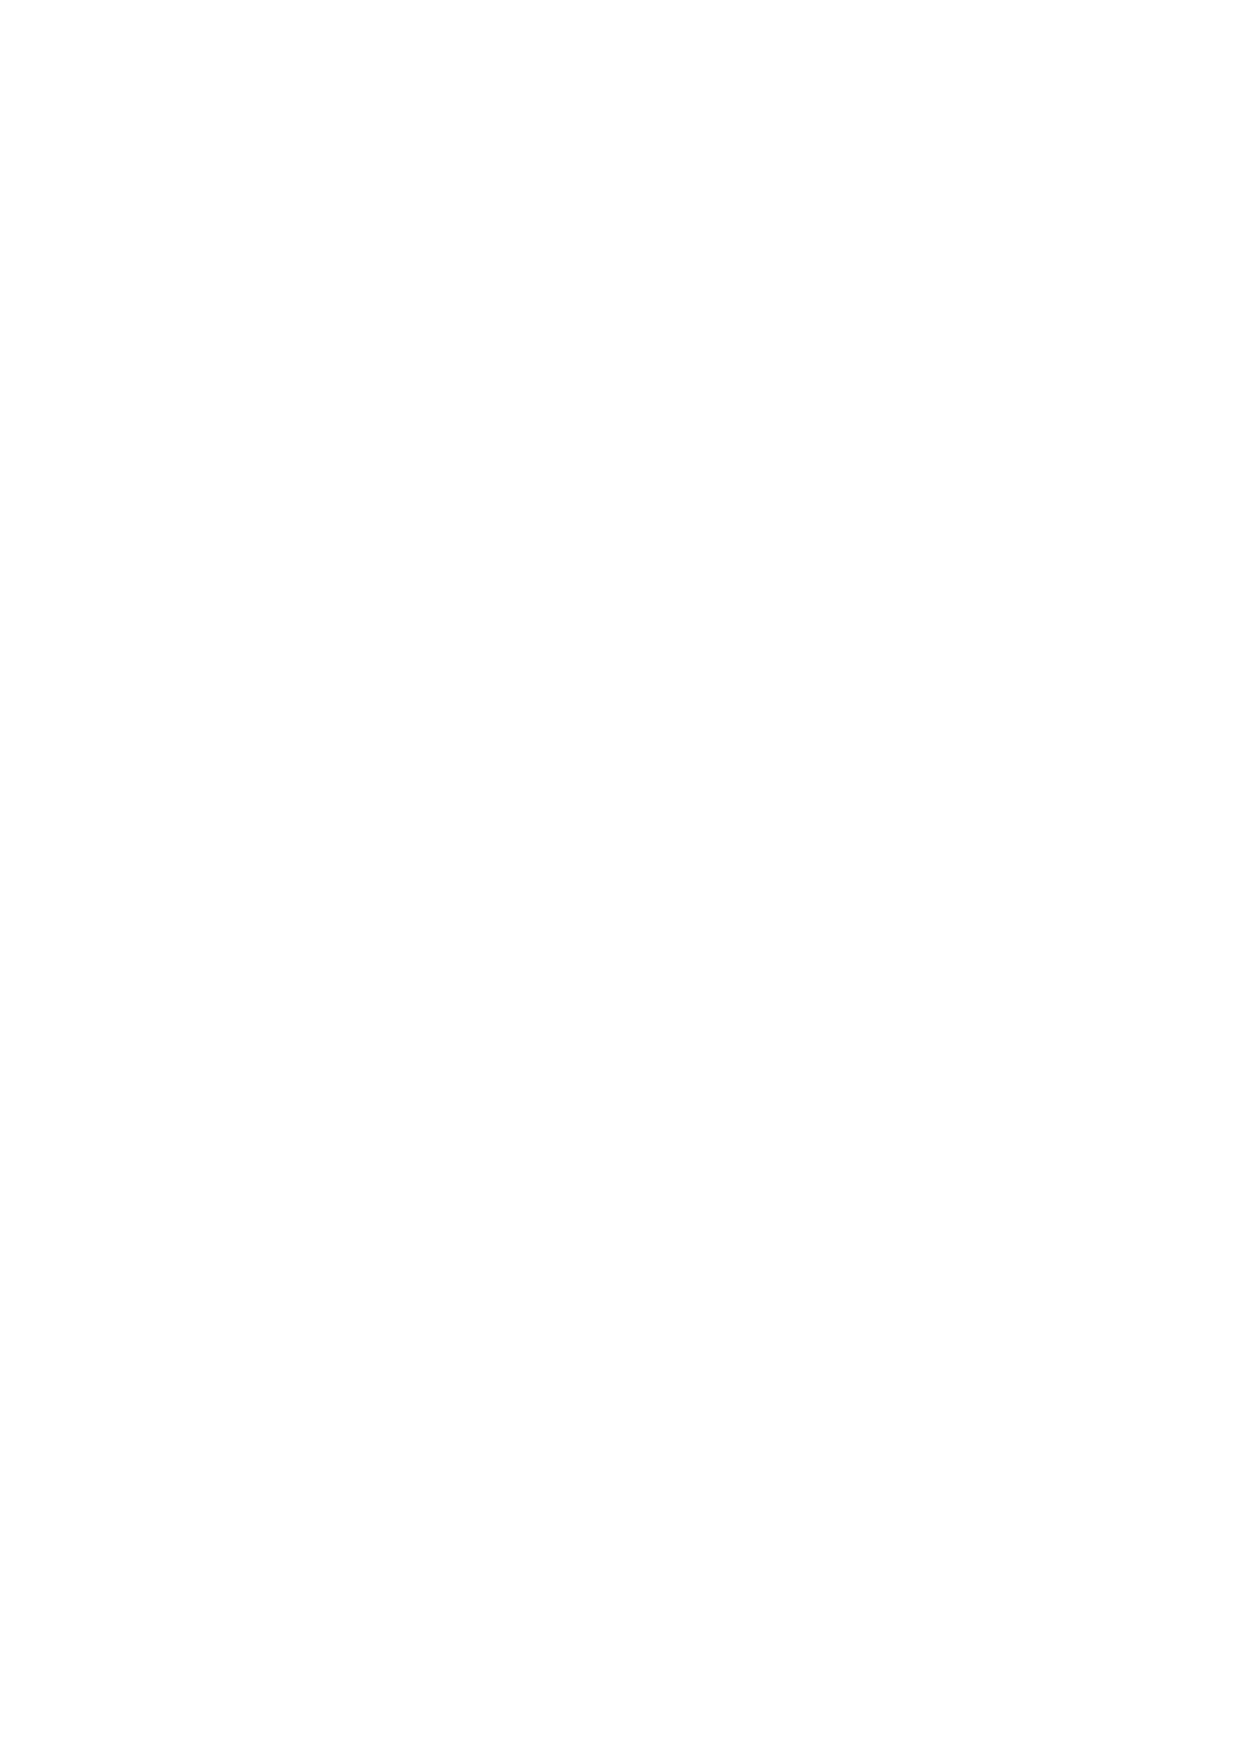
\includegraphics[]{\figs/clist} 
\end{figure}

\subsection{Double linked list}
\begin{itemize}
    \item In this linked list, each node has two pointers, one that points to the next node and the other that points to the previous node. 
    \item The previous pointer in the first node and the next pointer in the terminal node are always pointing to null. 
    \item This is a way of implementing a dynamic double ended queue. 
\end{itemize}
\begin{figure}[H]
    \centering
    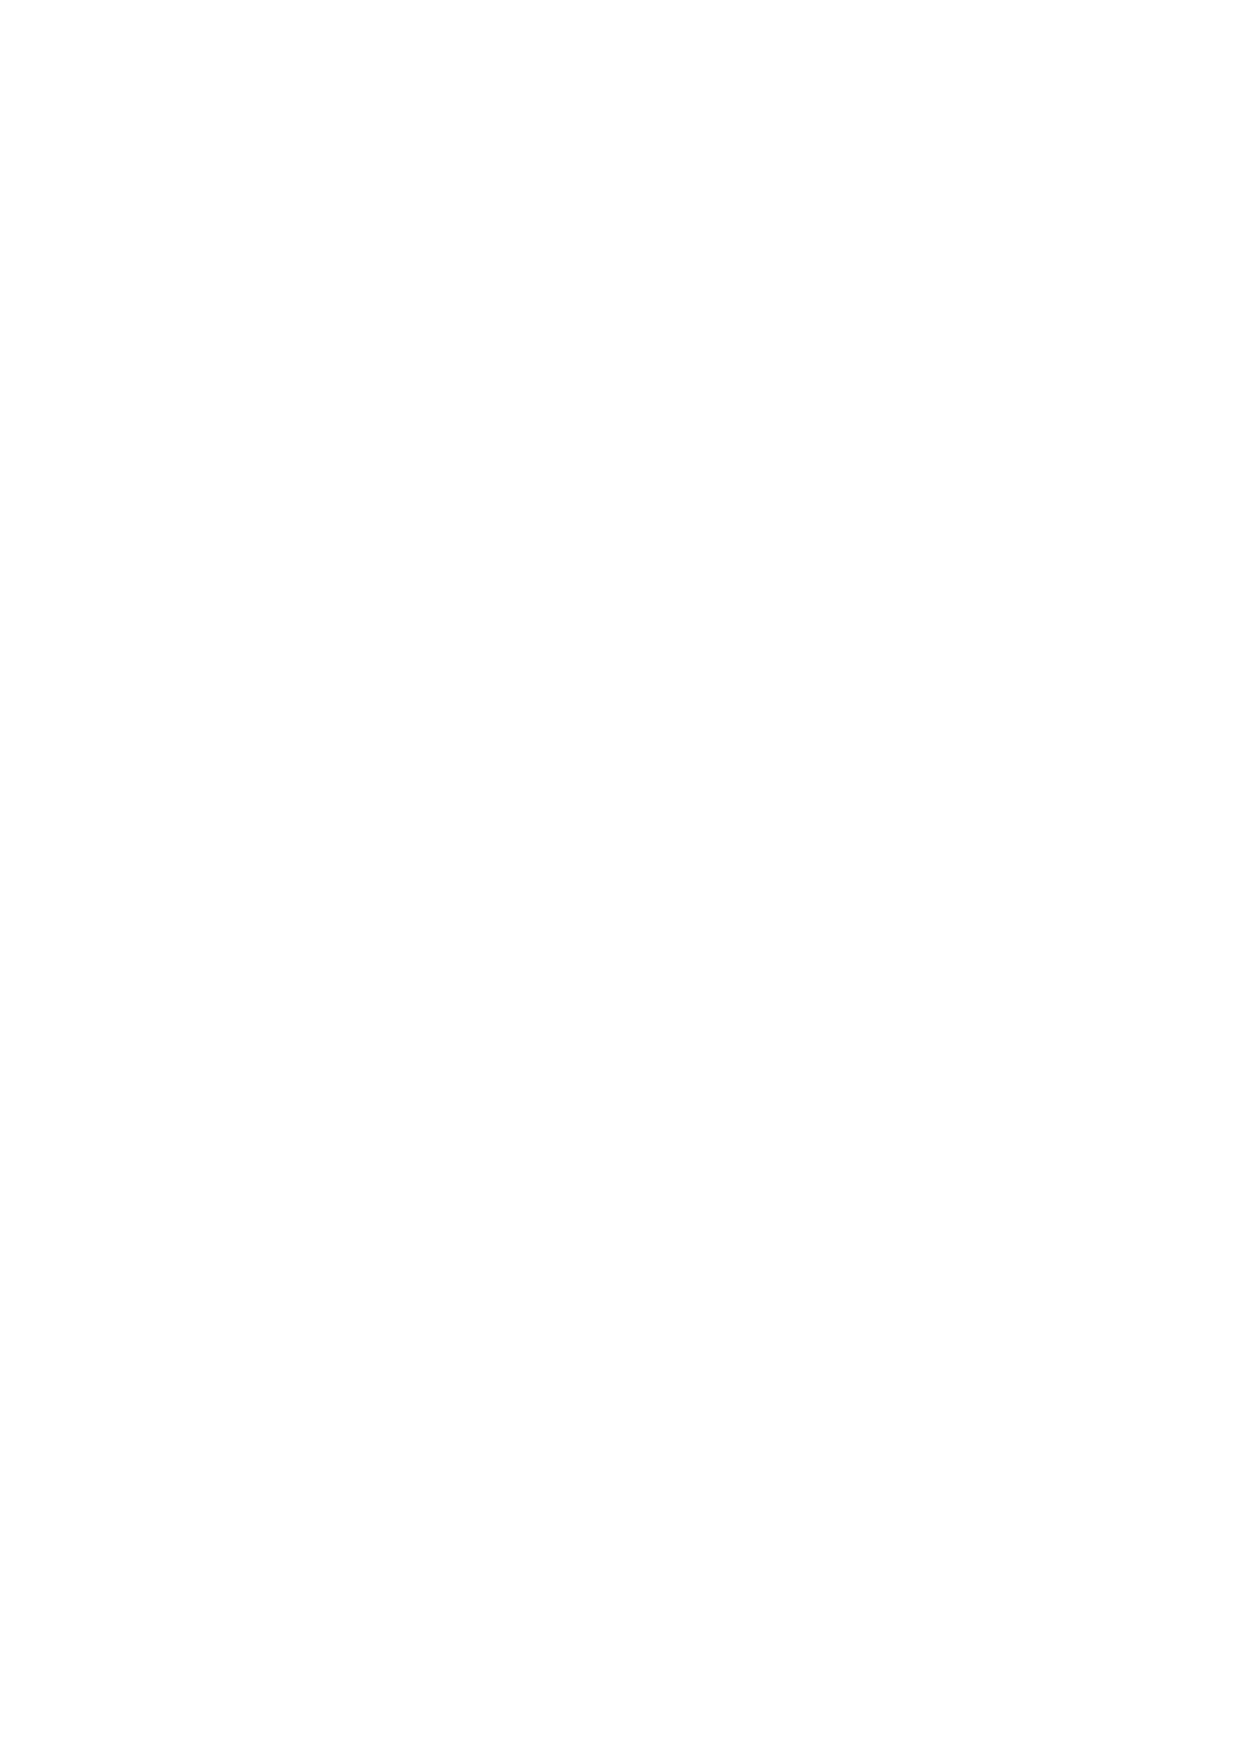
\includegraphics[]{\figs/dllintro} 
\end{figure}


\chapter{Variables and constants}
\section{Overview}
\begin{itemize}
    \item Statements are executed in the order they appear. 
    \item Control flow statements will break this order based on decision-making. 
    \item Code can be repeated; branching statements can execute only certain code, these are used inside loops; decision-making.  
\end{itemize}
\subsection{Decision-making}
\begin{itemize}
    \item Asks a question inside, the answer will respond. 
    \item If the condition is true a statement is executed, if not then the code isn't executed.  
\end{itemize}
If statements: 
\begin{center}
    \begin{tabular}{ |p{5cm}|p{7cm}| }
        \hline
            Statement & Description \\
        \hline \hline
            if statement & If statement consists of a boolean expression, followed by on or more statements. \\ 
        \hline
            if...else statement & if statements can be followed by else statements which executes when the boolean expression of the if statement is false \\ 
        \hline
            nested if statements & multiple conditions are evaluated, if statement inside a statement. \\ 
        \hline
    \end{tabular}
\end{center}
\subsection{Repeating code}
\begin{itemize}
    \item Loop statements allows us to repeat code. 
    \item When execution leaves a scope, all automatic objects that were created in that scope are destroyed. 
\end{itemize}
Loops   
\begin{center}
    \begin{tabular}{ |p{5cm}|p{7cm}| }
        \hline
            Loop type & Description \\
        \hline
            while & repeats until condition \\ 
            for & repeats a number of times \\ 
            do...while & while loop but with the exception that it tests the condition at the end of the loop body \\ 
            nested loops & using one inside another \\ 
        \hline
    \end{tabular}
\end{center}


%----------------------------------------------------------------------------------------
\section{If statements}
\subsection{if else}
\begin{itemize}
    \item Syntax is: \mintinline{c}{if (expression) { /*program statement */};}
    \item For compound statements you need to surround the program statement with curly braces, if only one statement is used it's okay to use it without the curly braces. 
\end{itemize}
If with an else: 
\begin{itemize}
    \item An addition to the if block, you can add an else clause. 
    \item Syntax is: \mintinline{c}{if (expression) statement; else statement;} 
\end{itemize}
\subsubsection{Example}
\inputcode{\lang}{\code/if_else_statements.c}

\subsection{else if}
\begin{itemize}
    \item To ask multiple questions. 
    \item Syntax is: 
        \begin{minted}[autogobble]{c}
            if (expression) /* program statement */; 
            else if (expression) /* program statement */; 
            else /* program statement */; 
        \end{minted}
\end{itemize}
\subsubsection{Example}
\inputcode{\lang}{\code/else_if_statement.c}

\subsection{nested if-else statement}
\begin{itemize}
    \item If or if else statement inside another. 
    \item Syntax is: 
        \begin{minted}[autogobble]{c}
            if (expression) {
                if (expression) {
                    statements;
                }
            }
        \end{minted}
\end{itemize}

\subsection{The conditional operator (ternary operator)}
\begin{itemize}
    \item This is equivalent to an if else statement. 
    \item Syntax is: \placeholder{\mintinline{c}{condition}}? \mintinline{c}{expression1: expression2;}|
    \item First operand is placed before the ?, the second after the ? and before the : and the third one after the : 
    \item This is a short hand notation for if else statements, there are no compound statements here, only simple. 
    \item Example: 
        \begin{minted}[autogobble]{c}
            x = y > 7 ? 25 : 50; 
        \end{minted}
    result in x being set to 25 if y is greater than 7 or to 50 otherwise. 
\end{itemize}
\subsubsection{Example}
\inputcode{\lang}{\code/ternary_operator.c}


%----------------------------------------------------------------------------------------
\section{Switch statement}
\begin{itemize}
    \item Serve the same purpose as an if, the difference is that is more organized and made for multiple alternatives rather than using else if multiple times. 
    \item else ifs can be prone to errors. 
    \item Switch are more efficient than else if. 
    \item Syntax is: 
        \begin{minted}[autogobble]{c}
            switch (expression) {
                case val_1: 
                    program statement; break;
                case val_2: 
                    program statement; break;
                case val_n: 
                    program statement; break;
                default: 
                    program statement; break;
            }
        \end{minted}
    
    \item The expression in the switch argument is the thing to check for. Cases are like if (val). Default means else.
    \item Cases must be constants or constant expression. 
    \item  When more than one statement is included they don't have to have curly braces surrounding the statement. 
    \item The break statement indicates the termination of a particular case and terminates the switch statement. It jumps out. If the expression is not mutually exclusive (more than one case will be true), don't put the break statements, otherwise put them, keep in mind that there must be one case that terminates the switch statement. This can cause bugs. 
    \item If none of the cases are true the default block is executed. 
\end{itemize}
\subsection{Example}
\inputcode{\lang}{\code/switch.c}
\inputcode{\lang}{\code/another_switch.c}
%----------------------------------------------------------------------------------------
\subsection{goto statement}
\begin{itemize}
    \item Used for jumping to a specific line of code.
    \item Has two parts, the goto and the label name.
    \item Label is named following the same convention used in naming a variable. 
    \item Example: goto part2; part2 is a label and it has to be labeled for the compiler to know what line you mean. 
    \item You can jump all around in your code.
\end{itemize}
\subsubsection{Example}
\inputcode{\lang}{\code/goto.c}

%----------------------------------------------------------------------------------------
\section{Challenge calculate week pay}
\inputcode{\lang}{\code/challenge_week_pay.c}


%----------------------------------------------------------------------------------------
\section{For loops }
\begin{itemize}
    \item Allows us to repeat code, this is a counter controlled loop because the number of iterations are predefined. 
    \item Sentinel loops execute an undefined number of times until a certain condition is met. 
    \item For simple statements you can omit the braces.
    \item Below C99 you must declare the counter variable outside the for loop.
    \item Syntax is: \mintinline{c}{for (starting condition; continuation condition; action per iteration) {statements;}}
    \item Example:  
        \begin{minted}[autogobble]{c}
            for (int i, j = 2; i <= 5; ++i, j += 2) 
                printf("%5d",i*j);
        \end{minted}
    \item If the action per iteration is not put, the for loop becomes an infinite loop. 
    \item Something like: \mintinline{c}{for (;;){statements;}}
\end{itemize}
\subsection{Example}
\inputcode{\lang}{\code/infinite_loops.c}


%----------------------------------------------------------------------------------------
\section{While loop, do while}
\subsection{While loops}
\begin{itemize}
    \item Mechanism to execute a set of statements as long as a condition is met.
    \item Syntax is: \mintinline{c}{while (expression) {statements;}}
    \item You don't need to put curly braces when you only have one statement. 
    \item If the loop is true the loop has to have a breaking mechanism so that it doesn't become an infinite loop.
    \item While loops are called pretest loop, it executes if a condition pre-evaluated results in true.
\end{itemize}
\subsection{do-while loops}
\begin{itemize}
    \item In the do while loop, you execute the code at least once, while loops execute code if the condition is true, do-while loops are going to execute the code at least once, never zero, regardless of the condition being true or false. 
    \item After the first iteration it will become a while loop. 
    \item The condition is at the bottom. This is called a post-test loop.
    \item Syntax is: \mintinline{c}{do{statement;}while(condition)}
    \item Example: 
        \begin{minted}[autogobble]{c}
            do { 
                // prompt for password; 
                // read user input; 
            } while (/*input not equal to password*/);
        \end{minted}
\end{itemize}
\subsubsection{Example}
\inputcode{\lang}{\code/do_while.c}

\subsection{Which loop to use}
\begin{itemize}
    \item If you want to execute it at least once unconditionally, use the do-while. 
    \item if you want to execute it while some condition is true then use a regular while loop. 
    \item Its a matter of taste, what you can do in a for loop you can do in a while loop. 
    \item \mintinline{c}{for(;test;)} is the same as \mintinline{c}{while (test)}.
\end{itemize}

\subsection{For loop and while loop equivalents}
For equivalent in a while loop. 
\begin{minted}[autogobble]{c}
    initalize; 
    while (test){
        body; 
        update;
    }
\end{minted}
Same as: 
\begin{minted}[autogobble]{c}
    for (initialize; test; update){ 
        update;
    }
\end{minted}

\begin{itemize}
    \item For loops are appropriate when the loop involves initializing and updating a variable. 
    \item A while loop is better when the conditions are otherwise. 
    \item Use the while loop for logic controlled loops and the for loop for counter controlled loops. 
\end{itemize}
%----------------------------------------------------------------------------------------
\section{Nested loops and loop control - break and continue}
\subsubsection{Nested loops}
\begin{itemize}
    \item Nested loops are loops inside loops. 
    \item You can have a while loop inside a for loop and vice versa, etc. 
\end{itemize}
\subsubsection{Continue statements}
\begin{itemize}
    \item It will skip that iteration, if a condition is met you can skip the iteration. 
\end{itemize}
\subsubsection{Example}
\inputcode{\lang}{\code/continue.c}
PS you can iterate through enums. 

\subsection{Break statement}
\begin{itemize}
    \item Breaks are used to jump out of loops, they are a way to stop execution of the current loop. 
    \item If you are breaking out of a nested loop, the break will only affect the innermost loop containing the break.
    \item Used to break out of the loop if a condition is met. 
    \item Switch statements also use the break keyword, they do the same things. 
\end{itemize}
\subsubsection{Example}
\inputcode{\lang}{\code/break.c}

%----------------------------------------------------------------------------------------
\section{Challenge guess the number}
\inputcode{\lang}{\code/challenge_guess_num.c}



\chapter{Arrays and vectors}
\section{Errors and exception handling}
\begin{itemize}
    \item try: code that will be attempted. 
    \item except: in case of error this will be executed.
    \item finally: this will always be executed regardless of the error. 
\end{itemize}
\begin{minted}[autogobble]{python}
    def add(n1,n2):
        return n1 + n2 

    add(1,input("Num2:"))
    # output: error

    try:
        add(1,input("Num2:"))
    except:
        print("Error")
    else: 
        print("excecute if except is not excecuted")
    finally:
        print("Done")
\end{minted}


%----------------------------------------------------------------------------------------
\section{Pylint overview}
\begin{itemize}
    \item Unit testing: test your code, makes sure your code still works. 
    \item pylint \& unittest 
    \item PEP-8 unit testing convention. 
\end{itemize}
pylint: run on command line: 
\begin{Verbatim}[breaklines=true, breakanywhere=true]
pylint myfile.py 
\end{Verbatim}


%----------------------------------------------------------------------------------------
\section{unittest: run on command line:} 
in the cap.py file: 
\begin{minted}[autogobble]{python}
    def cap_text(text):
        return text.title()
\end{minted}
on test.py:
\begin{minted}[autogobble]{python}
    import unittest
    import cap 
    class TestCap(unittest.TestCase): 
        def test_one_word(self):
            text = "python"
            result = cap.cap_text(text)
            self.assertEqual(result,"Python")
        def test_multiple_words(self): 
            text = "monty python"
            result = cap.cap_text(text)
            self.assertEqual(result,"Monty Python")
    if __name__ == "__main__":
        unittest.main()
\end{minted}


% \chapter{Statements and operators}
% \section{Introduction}
\begin{itemize}
    \item In a circular linked lists we have pretty much the same situation as a singly linked list, the difference is that we have only one pointer to the list, the tail, and the tail.next does not point to NULL, instead it points to the first element of the list. 
    \item We only keep track of the tail, considering the tail.next is the first node of the list.
    \item There is only one terminal node, no head, the tail will tell us everything we need to know. 
    \item The best use for a circular linked list is to build a circular queue. 
\end{itemize}

\subsection{Circular linked list visualization}
A populated circular linked list.
\begin{figure}[H]
    \centering
    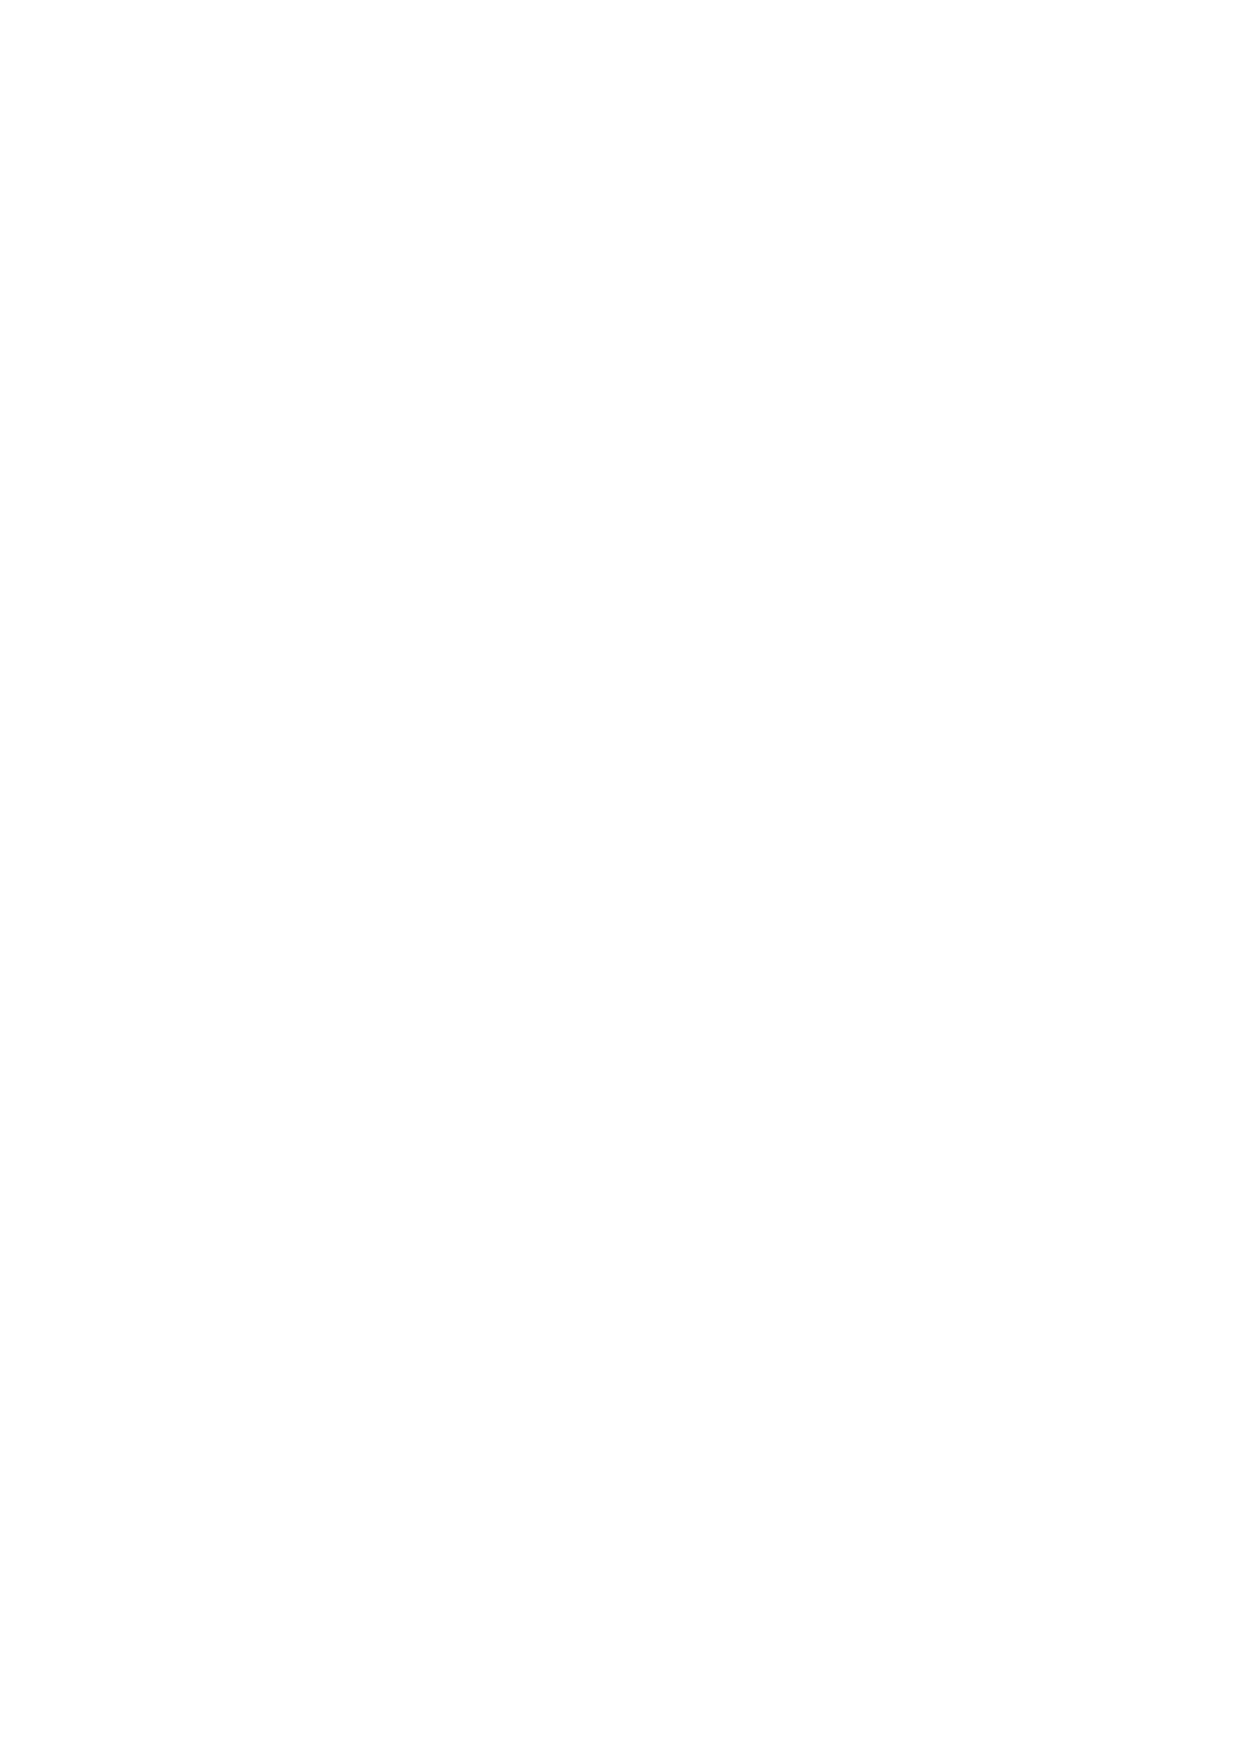
\includegraphics[
        % width=\textwidth, height={\textheight-1.2cm}, keepaspectratio
    ]{\figs/cll} 
\end{figure}
When there is only one node, the list looks like this.
\begin{figure}[H]
    \centering
    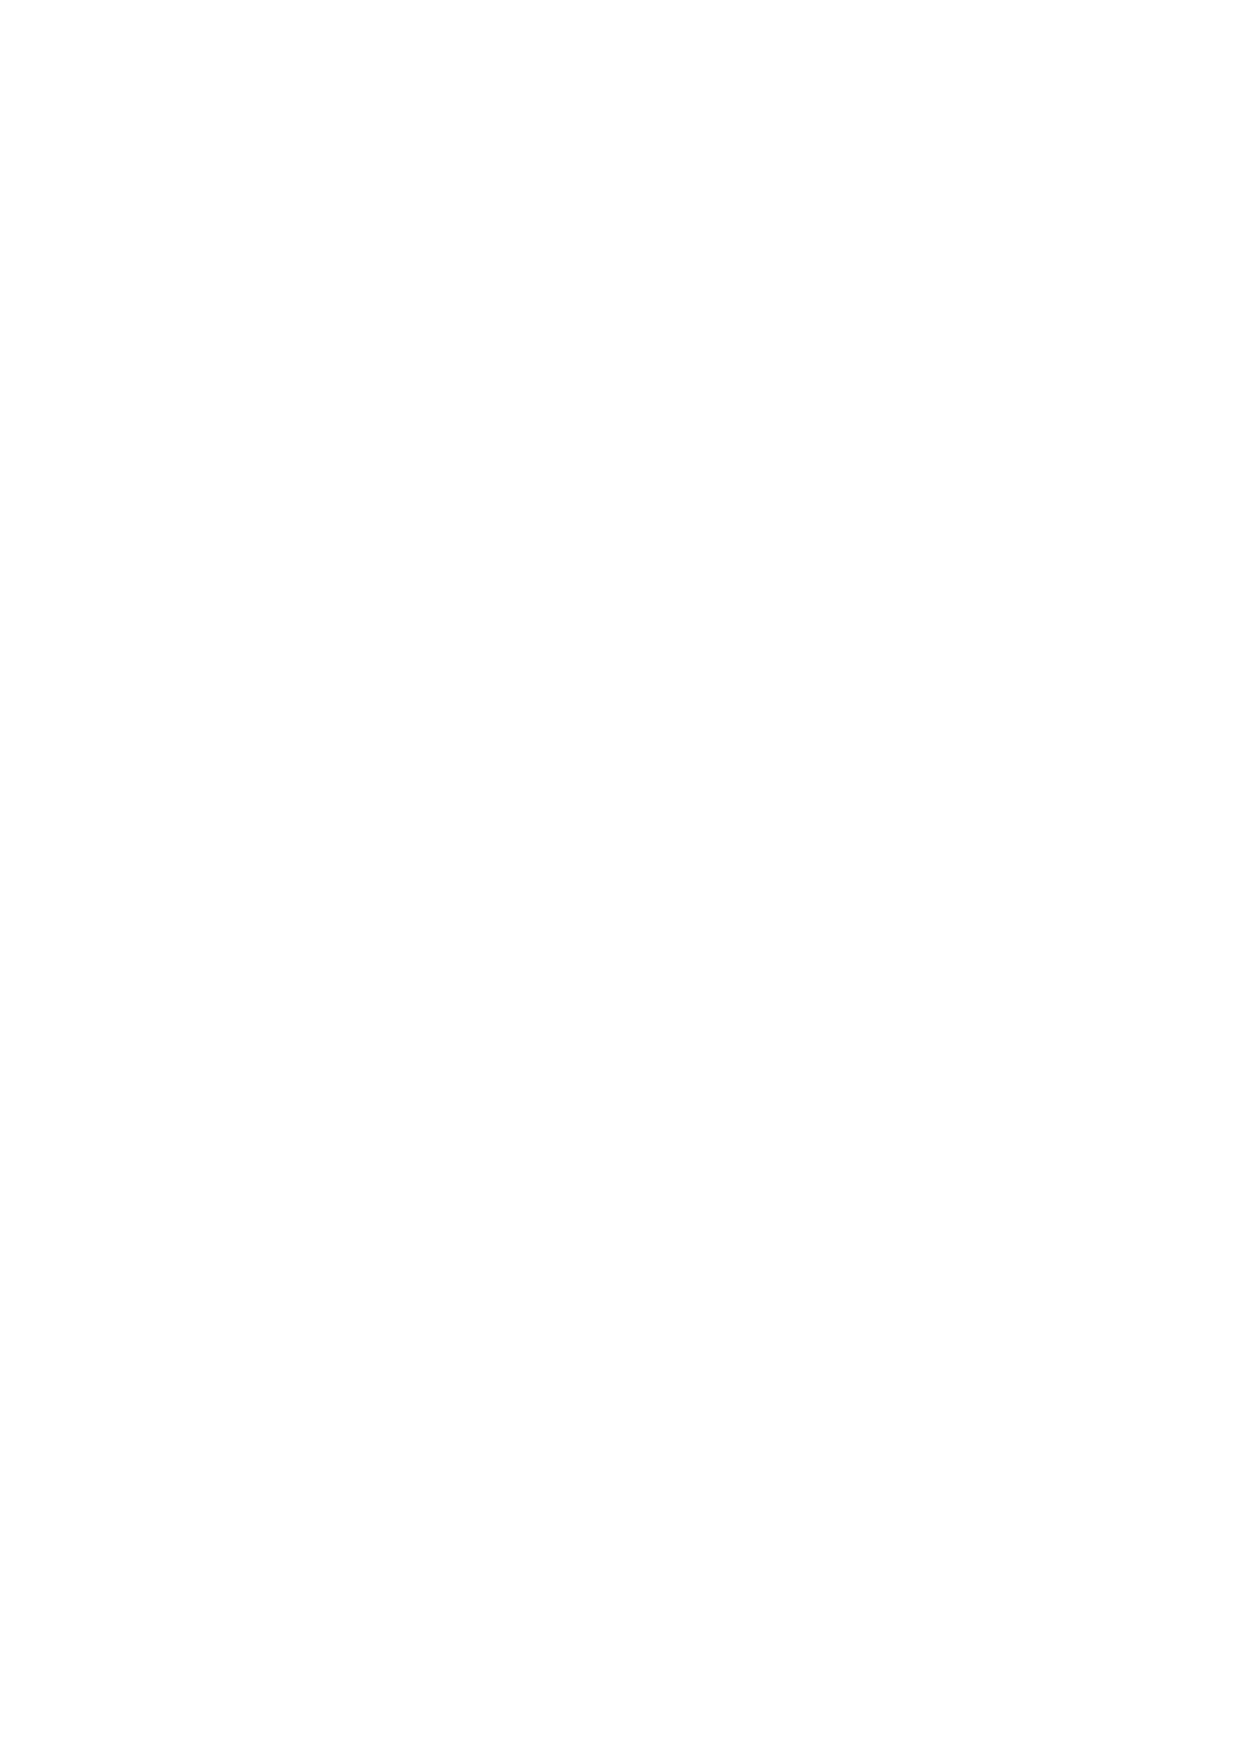
\includegraphics[
        % width=\textwidth, height={\textheight-1.2cm}, keepaspectratio
    ]{\figs/cllone} 
\end{figure}
\begin{itemize}
    \item When the list is empty the first node inserted will have a .next pointing to itself.
\end{itemize}

\section{Operation for inserting a node to circular linked list}
\begin{figure}[H]
    \centering
    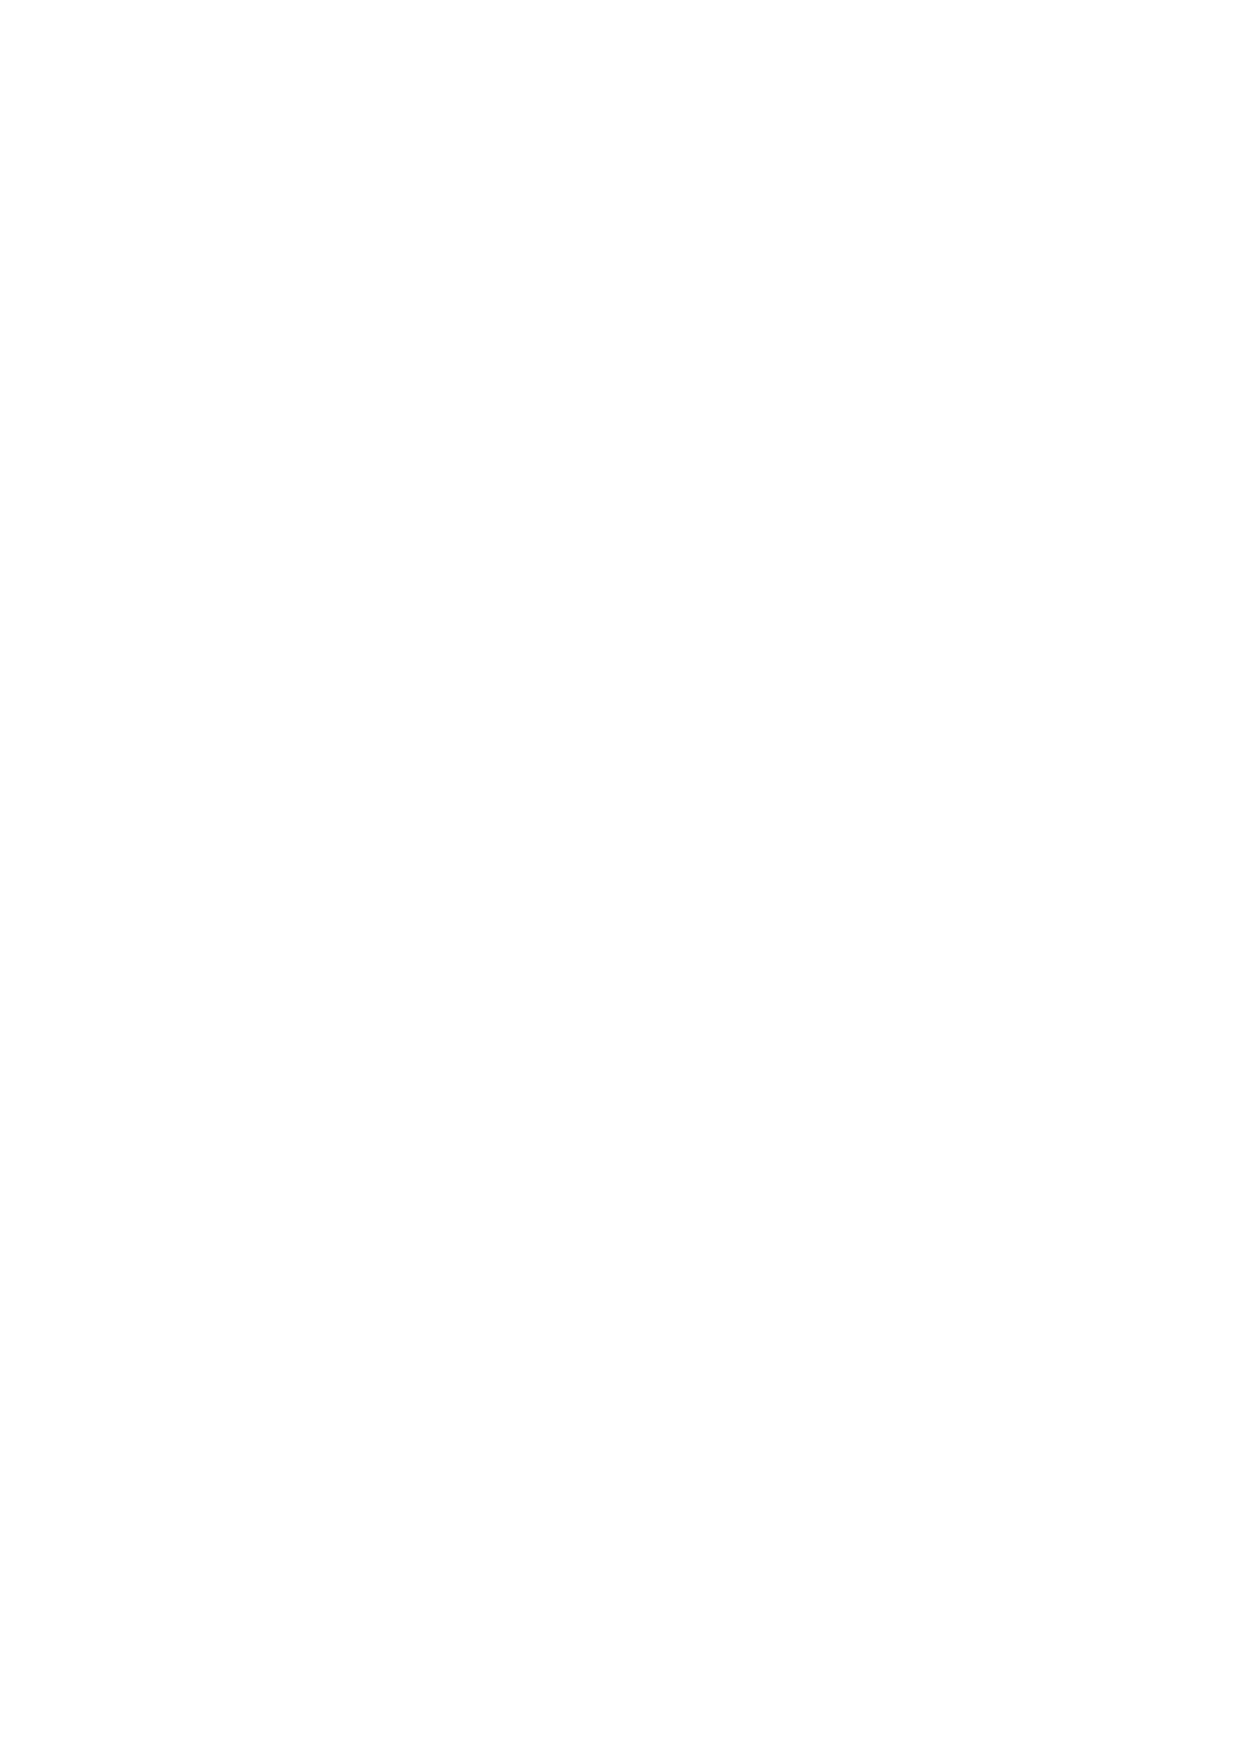
\includegraphics[
    width=\textwidth, height={\textheight-1.2cm}, keepaspectratio
                    ]{\figs/insertnodecll}
\end{figure}

\section{Operation for finding a target node in circular linked list}


\section{Operation for deleting a node in circular linked list}


\section{Operation for printing nodes in circular linked list}  



% \chapter{Controlling program flow}
% \section{Overview}
\begin{itemize}
    \item You can't put a char in double quotes, the compiler will interpret anything between double quotes is a string constant. 
    \item Single quotes = chars, Double quotes = strings.
    \item To display a double quote character use \mintinline{c}{\"}.
    \item The string in memory always one character more, this is a null character represented by \mintinline{c}{\0}.
    \item Null character with the code value 0 is added to the end of each string to mark where it ends in memory. \mintinline{c}{\0} character is always included. 
    \item The length of a string is always one greater than the number of characters in the string. 
    \item Don't confuse the null character with the null characters: 
        \begin{itemize}
            \item null character is a string terminator. 
            \item \mintinline{c}{NULL} is a symbol that represents a memory address that doesn't reference anything. 
        \end{itemize}
    
    \item You can add a \mintinline{c}{\0} character to a string explicitly, in this case it will create two strings. If you add \mintinline{c}{\0} to a string in the middle the string will only be counted or recognized up until that null character. 
\end{itemize}
\subsection{Example}
\inputcode{\lang}{\code/null_character.c}


%----------------------------------------------------------------------------------------
\section{Defining a string}
\begin{itemize}
    \item C doesn't have a special type for strings, this means you can't use any of the operators with C for strings, you'll have to use a library.  
    \item Strings in C are stored in an array of type char. 
    \item Character strings are stored in adjacent memory cells. 
    \item Example: \mintinline{c}{char my_str[20];} 19 chars taking in to account the \mintinline{c}{\0} character. 
    \item The compiler will add the null character automatically at the end of the string constant. 
\end{itemize}
Initializing: 
\begin{itemize}
    \item To initialize a character array you put the characters in between the brackets. 
    \item Example: 
        \mint{c}{char word[] = {'H','e','l','l','o','!'};}
    The compiler will automatically add the null character, declaring a char array like a string doesn't require a number of elements in between the square braces, the compiler will add that automatically. 
    
    \item Short hand notation: 
        \mint{c}{char word[] = {"Hello!"}; }
    Let the compiler figure out the size for you. Leave the braces empty. 
    
    \item You can also initialize just part of the array such as: \mintinline{c}{char str[40] = "To be";} 5 will be used, the others are actually empty. 
\end{itemize}
Assigning a value to a string after initializing: 
\begin{itemize}
    \item Since strings are arrays, you can't assign strings either. 
    \item Things such as the following are not allowed: 
        \begin{minted}[autogobble]{c}
            char s[100]; 
            s = "hello"; // error 
        \end{minted}
    
    \item You can't assign an array of characters to another array of characters. To do that use a special function from the string library called strncpy().
\end{itemize}
Displaying a string: 
\begin{itemize}
    \item To display a string with printf use the format specifier \%s: 
    \begin{Verbatim}[breaklines=true, breakanywhere=true]
        printf("\nThe message is: %s",message);
    \end{Verbatim}
    
    \item \%s expects a null terminated string. 
    \item To print a character array you can use the format specifier to format the printf(), using just the name of the character array, this is unique, this is the only type of array that enables this type of printing. 
\end{itemize}
Inputting a string: 
\begin{itemize}
    \item To input string using scanf():
        \begin{minted}[autogobble]{c}
            char input[10]; 
            printf("Please input your name");
            scanf("%s",input); // no ampersand because it's an array. 
        \end{minted}
    
    \item \%s is for inputting and outputing strings. 
    \item Don't use the \& in character arrays for scanf().
\end{itemize}
Testing if two strings are equal: 
\begin{itemize}
    \item You can't do this: \mintinline{c}{if (str1 == str2);}, strings are character arrays so operators can't be applied to them. Don't use == in strings. Remember "x" is two chars because of the null char, 'x' is just one. 
    \item If you wanted to check if two strings are equal you would actually have to use a for loop and compare each character, so there is a standard library function called strcmp(), use this to compare.
\end{itemize}

\subsection{Example}
\inputcode{\lang}{\code/defining_a_str.c}


%----------------------------------------------------------------------------------------
\section{Constant strings} 
\begin{itemize}
    \item the \#define is used to define constants, there are constant strings. 
    \item Constant strings remain hence the name, constant all throughout the program. You may want to use constant strings for readability. You can later change the constant string in one place instead of everywhere you used it. Avoid magic numbers, use constants. 
    \item \#define is a preprocessor statement to define constants. 
    \item Syntax is: \#define \placeholder{var\_name} \placeholder{value}, no semicolon or equals operator. 
    \item All \#define directives are globals, there is no thing as a local \#define.
    \item \#define can be used for char and string constants. 
        \begin{minted}[autogobble]{c}
            #define BEEP 'a'
            #define TEE 'T'
            #define ESC '\033'
            #define OPPS "Now you have done it" 
        \end{minted}
    
    \item Another way to create constant is to use the \mintinline{c}{const} keyword. This means data defined as \mintinline{c}{const} will not be able to change, its another equivalent for \#define. \verb|const| is a read-only value, you can use consts in calculations an whatever as long as you don't alter the value, this is not allowed. const can replace magic numbers. 
    \item Const is more flexible to \#define, it lets you declare a type and allows better control over whch parts of a program can use the constant, is to say that const can be local and global. 
    \item Example: \mintinline{c}{const int MONTHS = 12;}
    \item Third way to declare constants are using enums. 
    \item For initialization of a const string:
        \begin{minted}[autogobble]{c}
            const char message[] = "The end of the world is nigh.";
        \end{minted}
    
    \item Any attempt to modify it by doing a strcopy() will cause an error. 
\end{itemize}


%----------------------------------------------------------------------------------------
\section{String functions}
\begin{itemize}
    \item C standard library includes functions that can operate on strings. 
\end{itemize}
C standard functions on strings \mintinline{c}{#include <string.h>}: 
\begin{itemize}
    \item strlen(): getting length of string. 
        \begin{itemize}
            \item This functions does change the string, string is not parametrized as a constant. 
        \end{itemize}
    \inputcode{\lang}{\code/strlen.c}
    \item strcpy() and strncpy(): copying one character string to another. 
        \begin{itemize}
            \item \mintinline{c}{char s[100]; s = "hello";} doesn't work in C, you'll have to use strcpy()
            \item The strcpy() doesn't check the length of the character array, thus it's prone to errors such as out of bounds errors.
            \item The strncpy() takes in an third argument, the maximum number of characters to copy. 
        \end{itemize}
    \inputcode{\lang}{\code/strcpy.c}
    \item strcat() and strncat(): used for concatenation.
        \begin{itemize}
            \item strncat() takes consideration of the size of the string, strcat() doesn't. 
        \end{itemize}
    \inputcode{\lang}{\code/strcat_strncat.c}
    \item strcmp(): compare strings to see if they are equal. 
        \begin{itemize}
            \item str1 == str2 will compare whether the strings have the same address, not the actual content.  
            \item in strcmp(), if the result is 0 means that they are the same string, if the result is negative or positive they are not equal. 
            \item If the return is negative $\rightarrow$ str1 is less than str2. 
            \item If return is positive $\rightarrow$ str2 is less than str1.
            \item You don't have to worry about the size of arrays being compared thus no strncmp() not for ensuring no buffer overflows, its for comparing substrings. For example, you want all strings that start in ``astro'' you'll use strncmp(), use strncmp() when you are interested in prefixes.
        \end{itemize}
    \inputcode{\lang}{\code/strcmp_equal.c}
\end{itemize}
\subsection{String functions examples}
\inputcode{\lang}{\code/strlen_strncpy.c}


%----------------------------------------------------------------------------------------
\section{Searching, Tokenizing, and Analyzing Strings}
\begin{itemize}
    \item Searching a string: To find a single character or substring use: strchr() and strstr().
    \item Tokenizing: Sequence of characters within a string bounded by a delimeter (space,comma,period,etc); Breaking a sentence into words is called tokenizing. Use: strtok() 
    \item Analyzing strings: islower(), isupper(), isalpha(), etc. 
\end{itemize}

\subsection{Pointers}
\begin{itemize}
    \item A pointer is a useful type of variable, related to memory. A pointer is a variable that stores an address, its value is the address of another location in memory that can contain value. 
        \begin{minted}[autogobble]{c}
            int Number = 25; 
            int *pNumber = &Number; 
        \end{minted}
    
    \item *pNumber is a pointer, it points to address of Number. 
\end{itemize}
\begin{center}
    \begin{tabular}{ |c|c|c| }
        \hline
            Variable & Address & Value \\
        \hline \hline
            Number & 1000 & 25 \\ 
        \hline
            pNumber & 1004 & 1000 \\ 
        \hline
    \end{tabular}
\end{center}

\subsection{Searching a string for a character}
\begin{itemize}
    \item strchr() function searches a given string for a specified character. The first argument is the string to search (given as an address) and the second is the character to look for. 
    \item The function will return a pointer to the first position in the string where the character is found. The address to this position in memory and it is of type char* or ``pointer to char''.
    \item To store a value returned you must store it in a variable that can store the address of a character. 
    \item If the character is not found, the function returns a null value. For a pointer null represents a pointer that is not pointing to anything. 
\end{itemize}
\begin{minted}[autogobble]{c}
    char str[] = "The quick brown fox"; 
    char ch = 'q';
    char *pGot_char = NULL; 
    pGot_Char = strchr(str,ch); // pointer will be pointed to the q address. 
\end{minted}
\begin{itemize}
    \item In the example you can also use an int as a char to look for, it will be converted to ASCII equivalent. 
\end{itemize}

\subsection{Searching for a substring}
\begin{itemize}
    \item strstr() searches one string for the first occurrence of a substring. It returns a null pointer if non is found. 
    \item Returns a pointer to the position in the first string where the substring is found. 
    \item The search is case-sensitive. 
\end{itemize}
\begin{minted}[autogobble]{c}
    char text[] = "Every dog has his day";
    char word[] = "dog"; 
    char *pFound = NULL; 
    pFound = strstr(text,word);
\end{minted}

\subsection{Tokenizing a string}
\begin{itemize}
    \item Token is a sequence of characters within a string that is bound by a delimiter, the delimiter can be anything, best if the delimiter is something meaningful.
    \item strtok(): first argument is the string to be tokenized, a string containing all the possible delimiter characters. 
\end{itemize}
\inputcode{\lang}{\code/strtok.c}

\subsection{Analyzing strings}
\begin{itemize}
    \item \mintinline{c}{islower()}: lower case.
    \item \mintinline{c}{isupper()}: upper case.
    \item \mintinline{c}{isalpha()}: lower or upper case.
    \item \mintinline{c}{isalnum()}: upper case or lower case or a digit. 
    \item \mintinline{c}{iscntrl()}: control character. 
    \item \mintinline{c}{isprint()}: any printing character including a space. 
    \item \mintinline{c}{isgraph()}: any printing character except a space.
    \item \mintinline{c}{isdigit()}: decimal digit (0-9)
    \item \mintinline{c}{isxdigit()}: hexadecimal digit (0-9,A-F,a-f)
    \item \mintinline{c}{isblank()}: standard blank characters, space and \verb|\t|
    \item \mintinline{c}{isspace()}: white space character such as: \verb|space, \n, \t, \v, \r, \f|
    \item \mintinline{c}{ispunct()}: printing character for shitch isspace is isalnum return false. 
\end{itemize}
\inputcode{\lang}{\code/analyzing_str.c}


%----------------------------------------------------------------------------------------
\section{Converting strings}
\begin{itemize}
    \item Use toupper() and tolower(). 
    \item Syntax is: \mintinline{c}{for (int i = 0; (buff[i]=(char)toupper(buff[i])) != '\0'; ++i);}
    \item This loop will cover the entire string in the buff array to uppercase by stepping through the strung one character at a time. 
    \item toupper() returns a type int, thats why we convert it. 
\end{itemize}
\inputcode{\lang}{\code/str_toupper.c}
This is all included in the stdio.h.
\begin{center}
    \begin{tabular}{ |c|p{7cm}| }
        \hline
            Function & Returns \\
        \hline
            \mintinline{c}{atof()} & A value of type double that is produced from  the string argument. Infinity as a double value is recognized from the strings ``inf'' or ``INFINITY'' where any character can be in uppercase or lowercase and ``not a number'' is recognized from the string ``NAN'' in uppercase or lowercase. \\  
            \mintinline{c}{atoi()} & A value of type int that is produced from the string argument. \\  
            \mintinline{c}{atol()} & A value of type long that is produced from the string argument. \\  
            \mintinline{c}{atoll()} & A value of type long long that is produced from the string argument.  \\ 
            \mintinline{c}{strtod()} & A value of type double is produced from the initial part of the string specified by the first argument. The second argument is a pointer to a variable, ptr say, of type char* in which the fucntion will store the address of the first character following the substring that was converted to the double value. If no string was found that could be converted to type double, the variable ptr will contain the address passed as the first argument. \\ 
            \mintinline{c}{strof()} & A value of type float. In all other respects it works as strtod(). \\ 
            \mintinline{c}{strtold()} & A value of type long double. In all other respects it works as strtod(). \\ 
        \hline
    \end{tabular}
\end{center}
\inputcode{\lang}{\code/convertion_function_example.c}

%----------------------------------------------------------------------------------------

\section{Challenge - Understanding char arrays}
\inputcode{\lang}{\code/challenge_write_strlen_compare_concat.c}

\subsection{Reverse a string}
\inputcode{\lang}{\code/challenge_reverse_a_str.c}




% \chapter{Characters and strings}
% \section{SELECT statements and prompts}
\begin{itemize}
    \item Find all employees:
        \begin{minted}[autogobble]{sql}
            SELECT * FROM employee;
        \end{minted}
        \begin{figure}[H]
            \centering
            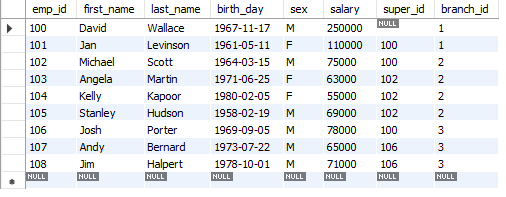
\includegraphics[width=0.4\textwidth]{./Figs/2020-12-24-20-38-38.png}
        % 	\caption{}
        \end{figure}
    
    \item Find all the clients:
        \begin{minted}[autogobble]{sql}
            SELECT * FROM client;
        \end{minted}
        \begin{figure}[H]
            \centering
            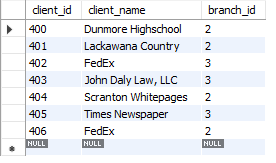
\includegraphics[width=0.4\textwidth]{./Figs/2020-12-24-20-39-09.png}
        % 	\caption{}
        \end{figure}
    
    \item Find all employees ordered by salary:
        \begin{minted}[autogobble]{sql}
            SELECT * FROM employee ORDER BY salary; 
        \end{minted}
        \begin{figure}[H]
            \centering
            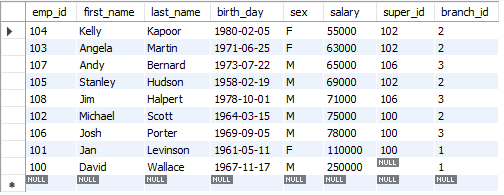
\includegraphics[width=0.4\textwidth]{./Figs/2020-12-24-20-39-36.png}
        % 	\caption{}
        \end{figure}
    
    \item Find all employees ordered by salary from largest to smallest and then smallest to largest:
        \begin{minted}[autogobble]{sql}
            SELECT * FROM employee ORDER BY salary DESC;
        \end{minted}
        \begin{figure}[H]
            \centering
            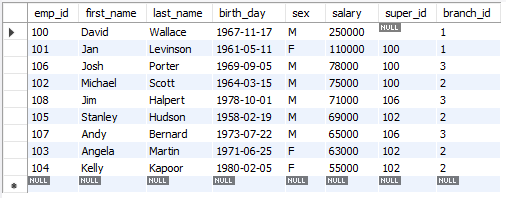
\includegraphics[width=0.4\textwidth]{./Figs/2020-12-24-20-44-00.png}
        % 	\caption{}
        \end{figure}
        \begin{minted}[autogobble]{sql}
            SELECT * FROM employee ORDER BY salary ASC;
        \end{minted}
        \begin{figure}[H]
            \centering
            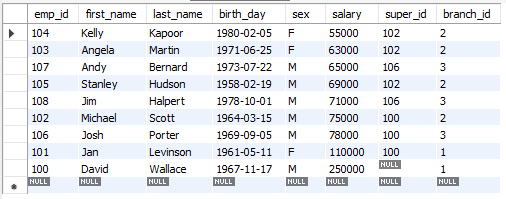
\includegraphics[width=0.4\textwidth]{./Figs/2020-12-24-20-44-41.png}
        % 	\caption{}
        \end{figure}
    
    \item Order all employees ordered by sex and then name:
        \begin{minted}[autogobble]{sql}
            SELECT * FROM employee ORDER BY sex, first_name, last_name; 
        \end{minted}
        \begin{figure}[H]
            \centering
            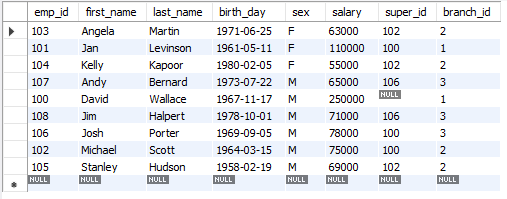
\includegraphics[width=0.4\textwidth]{./Figs/2020-12-24-20-43-11.png}
        % 	\caption{}
        \end{figure}
    
    \item Find the first 5 employees in the table:
        \begin{minted}[autogobble]{sql}
            SELECT * FROM employee LIMIT 5;
        \end{minted}
        \begin{figure}[H]
            \centering
            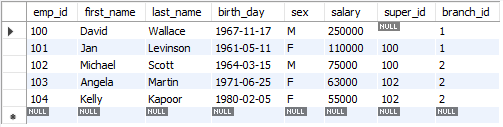
\includegraphics[width=0.4\textwidth]{./Figs/2020-12-24-20-45-25.png}
        % 	\caption{}
        \end{figure}
    
    \item Find the first and last names of all employees:
        \begin{minted}[autogobble]{sql}
            SELECT first_name, last_name FROM employee;
        \end{minted}
        \begin{figure}[H]
            \centering
            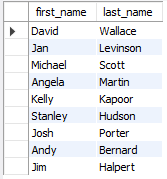
\includegraphics[width=0.4\textwidth]{./Figs/2020-12-24-20-45-46.png}
        % 	\caption{}
        \end{figure}
    
    \item  Find the forename and surnames of all employees:
        \begin{minted}[autogobble]{sql}
            SELECT first_name AS forename, last_name AS surname FROM employee;
        \end{minted}
        \begin{figure}[H]
            \centering
            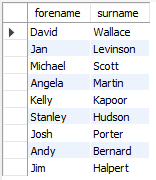
\includegraphics[width=0.4\textwidth]{./Figs/2020-12-24-20-46-18.png}
        % 	\caption{}
        \end{figure}
        \begin{itemize}
            \item \mintinline{sql}{AS} Allows you to select the columns differently to their names.
        \end{itemize}
    
    \item Find out all the different genders:
        \begin{minted}[autogobble]{sql}
            SELECT  DISTINCT sex FROM employee;
        \end{minted}
        \begin{figure}[H]
            \centering
            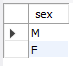
\includegraphics[width=0.4\textwidth]{./Figs/2020-12-24-20-46-37.png}
        % 	\caption{}
        \end{figure}
        \begin{itemize}
            \item \mintinline{sql}{DISTINCT} allows you to know all the values stored in a column. 
        \end{itemize}
    
    \item Find all male employees:
        \begin{minted}[autogobble]{sql}
            SELECT * FROM employee WHERE sex = 'M';
        \end{minted}
        \begin{figure}[H]
            \centering
            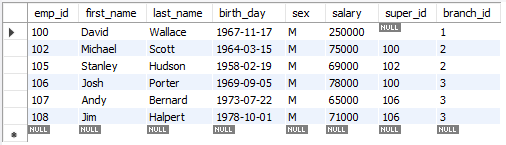
\includegraphics[width=0.4\textwidth]{./Figs/2020-12-24-20-47-19.png}
        % 	\caption{}
        \end{figure}
    
    \item Find all employees at branch 2:
        \begin{minted}[autogobble]{sql}
            SELECT * FROM employee WHERE branch_id = 2;
        \end{minted}
        \begin{figure}[H]
            \centering
            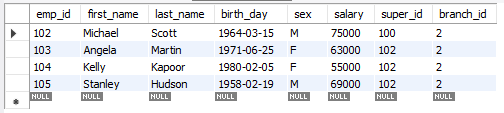
\includegraphics[width=0.4\textwidth]{./Figs/2020-12-24-20-48-13.png}
        % 	\caption{}
        \end{figure}
    
    \item Find all employee's id's and names who were born after 1969:
        \begin{minted}[autogobble]{sql}
            SELECT emp_id, first_name, last_name FROM employee WHERE birth_day >= 1970-01-01;
        \end{minted}
        \begin{figure}[H]
            \centering
            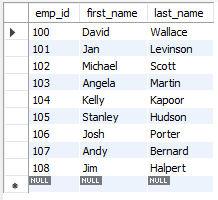
\includegraphics[width=0.4\textwidth]{./Figs/2020-12-24-20-48-48.png}
        % 	\caption{}
        \end{figure}
    
    \item Find all female employees at branch 2:
        \begin{minted}[autogobble]{sql}
            SELECT * FROM employee WHERE branch_id = 2 AND sex = 'F';
        \end{minted}
        \begin{figure}[H]
            \centering
            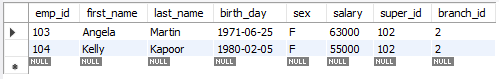
\includegraphics[width=0.4\textwidth]{./Figs/2020-12-24-20-49-50.png}
        % 	\caption{}
        \end{figure}
    
    \item Find all employees who are female  \& born after 1969 or who make over 80000:
        \begin{minted}[autogobble]{sql}
            SELECT * FROM employee WHERE (birth_day >= '1970-01-01' AND sex = 'F') OR salary > 80000;
        \end{minted}
        \begin{figure}[H]
            \centering
            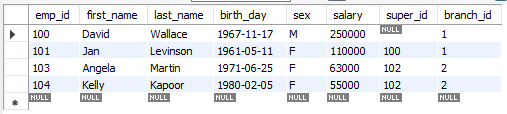
\includegraphics[width=0.4\textwidth]{./Figs/2020-12-24-20-50-39.png}
        % 	\caption{}
        \end{figure}
    
    \item Find all employees born between 1970 and 1975:
        \begin{minted}[autogobble]{sql}
            SELECT * FROM employee WHERE birth_day BETWEEN '1970-01-01' AND '1975-01-01';
        \end{minted}
        \begin{figure}[H]
            \centering
            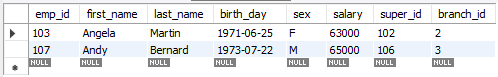
\includegraphics[width=0.4\textwidth]{./Figs/2020-12-24-20-51-24.png}
        % 	\caption{}
        \end{figure}
    
    \item Find all employees named Jim, Michael, Johnny or David:
        \begin{minted}[autogobble]{sql}
            SELECT * FROM employee WHERE first_name IN ('Jim', 'Michael', 'Johnny', 'David');
        \end{minted}
        \begin{figure}[H]
            \centering
            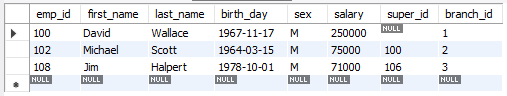
\includegraphics[width=0.4\textwidth]{./Figs/2020-12-24-20-52-10.png}
        % 	\caption{}
        \end{figure}
\end{itemize}



% \chapter{Functions}
% \section{Prompts to functions}
\begin{itemize}
    \item Find the number of employees are inside the employee table:
        \begin{minted}[autogobble]{sql}
            SELECT COUNT(emp_id) FROM employee;
        \end{minted}
    
    \item Find how many employees have supervisors:
        \begin{minted}[autogobble]{sql}
            SELECT COUNT(super_id) FROM employee;
        \end{minted}
    
    \item Find the number of female employees born after 1970:
        \begin{minted}[autogobble]{sql}
            SELECT COUNT(emp_id) FROM employee WHERE sex = 'F' AND birth_date > '1971-01-01';
        \end{minted}
    
    \item Find the average of all employee's salaries:
        \begin{minted}[autogobble]{sql}
            SELECT AVG(salary) FROM employee;
        \end{minted}
    
    \item Find the average of all employee's salaries who are male:
        \begin{minted}[autogobble]{sql}
            SELECT AVG(salary) FROM employee WHERE sex = 'M';
        \end{minted}
    
    \item Find the sum of all employee's salaries:
        \begin{minted}[autogobble]{sql}
            SELECT SUM(salary) FROM employee;
        \end{minted}
    
    \item Find out how many males and how many females there are:
        \begin{minted}[autogobble]{sql}
            SELECT COUNT(sex), sex FROM employee GROUP BY sex;
        \end{minted}
        \begin{itemize}
            \item This is called aggregation.
            \item The \mintinline{sql}{GROUP BY} allows us to display the count(sex) and sex in columns so that we can see what number belongs to what.
        \end{itemize}
    
    \item Find the total sales of each salesman:
        \begin{minted}[autogobble]{sql}
            SELECT SUM(total_sales), emp_id FROM works_with GROUP BY emp_id;
        \end{minted}
    
    \item Find the total purchases made from clients:
        \begin{minted}[autogobble]{sql}
            SELECT SUM(total_sales), emp_id FROM works_with GROUP BY client_id;
        \end{minted}
\end{itemize}
 

% \chapter{Pointers and references}
% \section{What is a pointer?}
\begin{itemize}
    \item A variable.
        \begin{itemize}
            \item Whose value is an address.
        \end{itemize}

    \item What can be at that address?
        \begin{itemize}
            \item Another variable.
            \item A function.
        \end{itemize}
    
    \item Pointers have a memory location that is bound to, type and has a value, this value is address in memory.
    \item If x is an integer variable and its value is 10 then I can declare a pointer that points to it.
    \item To use the data that the pointer is pointing to you must know its type.
\end{itemize}

\subsection{Why use pointers?}
\begin{itemize}
    \item Can't I just use the variable or the function itself?
        \begin{itemize}
            \item Yes, but you can't always do that.
        \end{itemize}
    
    \item Inside functions, pointers can be used to access data that are defined outside the function. Those values may not be in scope so you can't access them by their name.
    \item Pointers can be used to operate on arrays very efficiently.
    \item We can allocate memory dynamically on the heap or free store.
        \begin{itemize}
            \item This memory doesn't even have a variable name.
            \item The only way to get to it is via a pointer.
        \end{itemize}
    
    \item With object-oriented programming,  pointers are how polymorphism works.
    \item Can access specific addresses in memory.
        \begin{itemize}
            \item Useful in embedded and system applications.
        \end{itemize}
\end{itemize}


%----------------------------------------------------------------------------------------
\section{Declaring pointer variables}
\begin{itemize}
    \item We declare pointer variables in very much the same way any other variable would, except an asterisk must be between the type and the identifier:
        \begin{verbatim}
            variable_type *pointer_name;
        \end{verbatim}
        \begin{minted}[autogobble]{cpp}
            int *int_ptr; // pointer to int.
            double *double_ptr; // pointer to double.
            char *char_ptr; // pointer char.
            std::string *string_ptr; // pointer to a std::string.
        \end{minted}
        \begin{itemize}
            \item Keep in mind that there are many conventions to declaration of pointers, such as the one where the asterisk is next to the type \mintinline{cpp}{int* name;}, others where the asterisk is previous to the name \mintinline{cpp}{int *name;} or even a space from each \mintinline{cpp}{int * name;}
        \end{itemize}
    
    \item Intializing pointer variables to ``point no where'' or null:
        \begin{itemize}
            \item If you don't initialize your pointers they will have garbage data.
            \item In this case that data will be addresses.
            \item Just as an int was as convention initialized to a value, say 0, a pointer is usually initialized to null which means it doesn't point to any memory location. 
            \item You do this with the \mintinline{cpp}{nullptr} or the \mintinline{cpp}{NULL} keywords.
        \end{itemize}
        \begin{verbatim}
            variable_type *pointer_name {nullptr};
        \end{verbatim}
        \begin{minted}[autogobble]{cpp}
            int *int_ptr {};
            double *double_ptr {nullptr};
            char *char_ptr {nullptr};
            string *string_ptr {nullptr};
        \end{minted}
    
    \item Always initialize variable pointers to 'point no where 'or null.
        \begin{itemize}
            \item Always initialize.
            \item Uninitialized pointers contain garbage data and can 'point anywhere' in memory.
            \item Initializing to zero or \mintinline{cpp}{nullptr} (C++11) represents address zero.
                \begin{itemize}
                    \item Implies that the pointer is 'pointing nowhere'.
                \end{itemize}
            
            \item If you don't initialize a pointer to point to a variable or function then you should initialize it to \mintinline{cpp}{nullptr} to 'make it null'.
        \end{itemize}
\end{itemize}


%----------------------------------------------------------------------------------------
\section{Accessing the pointer address and storing address in a pointer}
\begin{itemize}
    \item The address operator.
        \begin{itemize}
            \item Variables are stored in unique addresses.
            \item Unary operator.
            \item Evaluates to the address of its operand.
                \begin{itemize}
                    \item Operand cannot be a constant or expression that evaluates to temp values.
                \end{itemize}
        \end{itemize}
        \begin{minted}[autogobble]{cpp}
            #include <iostream>
            using namespace std;
            int main() {
                int num{10};
                cout << "Value of num is: " << num << endl;
                cout << "Size of num is: " << sizeof num << endl;
                cout << "Address of num is: " << &num << endl;
                return 0;
            }
            /* OUTPUT:
            Value of num is: 10
            Size of num is: 4
            Address of num is: 0x61fe1c
            */
        \end{minted}
    
    \item Example:
        \begin{minted}[autogobble]{cpp}
            #include <iostream>
            using namespace std;
            int main() {
                int *p;
                cout << "Value of p is: " << p << endl; // garbage data.
                cout << "Address of p is: " << &p << endl; // value of p.
                cout << "Size of p is: " << sizeof p << endl; // size of p.
                p = nullptr;
                cout << "Value of p is: " << p << endl;
                return 0;
            }
            /* OUTPUT:
            Value of p is: 0x10
            Address of p is: 0x61fe18
            Size of p is: 8
            Value of p is: 0

            */
        \end{minted}
\end{itemize}

\subsection{sizeof a pointer variable}
\begin{itemize}
    \item Don't confuse the size of a pointer variable and the size of what it points to.
    \item All pointers in a program have the same size.
    \item They may be pointing to a very large or very small types.
\end{itemize}
\begin{minted}[autogobble]{cpp}
    int *p1 {nullptr};
    double *p2 {nullptr};
    unsigned long long *p3 {nullptr};
    vector<string> *p4 {nullptr};
    string *p5 {nullptr};
\end{minted}

\subsection{Storing an address in a pointer variable?}
Typed pointers.
\begin{itemize}
    \item The compiler will make sure that the address stored in a pointer variable is of the correct type.
\end{itemize}
\begin{minted}[autogobble]{cpp}
    int score {10};
    double high_temp {100.7};
    int *score_ptr {nullptr};
    score_ptr = &score;
    score_ptr = &high_temp; // compiler error because high_temp is a double and score_ptr is an int.
\end{minted}

\subsection{\& the address of operator}
\begin{itemize}
    \item Pointers are variables so they can change.
    \item Pointers can be null.
    \item Pointers can be uninitialized.
\end{itemize}



%----------------------------------------------------------------------------------------
\section{Dereferencing the pointer}
\begin{itemize}
    \item Access the data we're pointing to is called dereferencing a pointer.
    \item If \verb|score_ptr| is a pointer and has a valid address.
    \item Then you can access the data at the address contained in the \verb|score_ptr| using the dereferencing operator.
        \begin{minted}[autogobble]{cpp}
            #include <iostream>
            using namespace std;
            int main() {
                int score {100};
                int *score_ptr {&score};
                cout << *score_ptr << endl; // 100
                *score_ptr = 200;
                cout << *score_ptr << endl;
                cout << score << endl;
                return 0;
            }
            /* OUTPUT:
            100
            200
            200
            */
        \end{minted}
        \begin{itemize}
            \item Declaring and dereferencing is done using the asterisk, C++ has received some criticism about this, but once you understand where and how to use the asterisk you'll be fine.
        \end{itemize}

    
    \item Example:
        \begin{minted}[autogobble]{cpp}
            #include <iostream>
            #include <vector>
            using namespace std;
            int main() {
                vector<string> stooges {"Larry", "Moe", "Curly"};
                vector<string> *vector_ptr {nullptr};
                vector_ptr = &stooges;
                cout << "First stooge: " << (*vector_ptr).at(0) << endl;
                cout << "Stooges: ";
                for (auto stooge: *vector_ptr) {
                    cout << stooge << " ";
                }
                cout << endl;
                return 0;
            }
            /* OUTPUT:
            First stooge: Larry
            Stooges: Larry Moe Curly
            */
        \end{minted}
\end{itemize}


%----------------------------------------------------------------------------------------
\section{Dynamic Memory Allocation}
\begin{itemize}
    \item Allocating storage from the heap at runtime.
    \item We often don't knot how much storage we need until we need it.
    \item We can allocate storage for a variable at run time.
    \item Recall C++ arrays:
        \begin{itemize}
            \item We had to explicitly provide the size and it was fixed.
            \item But vectors grow and shrink dynamically.
        \end{itemize}
    
    \item We can use pointers to access newly allocated heap storage.
\end{itemize}

\subsection{Allocating and deallocating memory}
\begin{itemize}
    \item The \mintinline{cpp}{new} keyword
        \begin{itemize}
            \item Using the new keyword to allocate storage.
            \begin{minted}[autogobble]{cpp}
                #include <iostream>
                using namespace std;
                int main() {
                    int *int_ptr {nullptr};
                    int_ptr = new int; // allocate an integer on the heap.
                    cout << int_ptr << endl; // address of int_ptr.
                    cout << *int_ptr << endl; // garbage. Notice the dereferencing.
                    *int_ptr = 100;
                    cout << *int_ptr << endl; // 100.
                    return 0;
                }
                /* OUTPUT:
                0x25824f0
                39331936
                100
                */
            \end{minted}
    
        \item If you loose the pointer because it goes out of scope or other such incidents, that is called a memory leak and you lost the only way you have to access that memory.
        \item You also must deallocate the pointer after you are done using it.
        \end{itemize}
    
    \item The \mintinline{cpp}{delete} keyword
        \begin{itemize}
            \item The delete keyword is used to deallocate allocated space.
                \begin{minted}[autogobble]{cpp}
                    int *int_ptr {nullptr}; // allocate an integer on the heap.
                    delete int_ptr; // frees the allocated storage.
                \end{minted}
        \end{itemize}
    
    \item The \mintinline{cpp}{new[]} keyword
        \begin{itemize}
            \item The \mintinline{cpp}{new[]} is used to allocate an array.
                \begin{minted}[autogobble]{cpp}
                    int *array_ptr {nullptr};
                    int size {};
                    cout << "How big do you want the array: ";
                    cin >> size;
                    array_ptr = new int[size]; // allocate array on the heap.
                \end{minted}
            \item Keep in mind that these brackets must be empty.
        \end{itemize}
    

    \item The \mintinline{cpp}{delete[]} keyword is used to deallocate storage of an array.
        \begin{minted}[autogobble]{cpp}
            int *array_ptr {nullptr};
            int size {};
            cout << "How big do you want the array: ";
            cin >> size;
            array_ptr = new int[size]; // allocate array on the heap.
            delete[] array_ptr; // free allocated storage.
        \end{minted}
        \begin{itemize}
            \item Keep in mind that these brackets must be empty.
        \end{itemize}
    
    \item When you allocate dynamically you are allocating into the heap or the free store, the stack houses the pointer to the dynamically allocated data.
        \begin{itemize}
            \item Example:
                \begin{minted}[autogobble]{cpp}
                    #include <iostream>
                    using namespace std;
                    int main() {
                        size_t size{0}; // allocated on the stack.
                        double *temp_ptr {nullptr}; // allocated on the stack.
                        cout << "How many temps: "; 
                        cin >> size;
                        temp_ptr = new double[size]; // allocated on the heap.
                        cout << temp_ptr << endl;
                        delete[] temp_ptr; // dealocated on the heap.
                        return 0;
                    }
                \end{minted}
        \end{itemize}
\end{itemize}



%----------------------------------------------------------------------------------------
\section{Relationship between arrays and pointers}
\begin{itemize}
    \item The value of an array name is the address of the first element in the array.
    \item The value of a pointer variable is an address.
    \item If the pointer points to the same data types as the array element then the pointer and array name can be used interchangeably (almost).
        \begin{minted}[autogobble]{cpp}
            #include <iostream>
            using namespace std;
            int main() {
                int scores[] {100,95,89};
                cout << scores << endl;
                cout << *scores << endl;
                int *score_ptr {scores};
                cout << score_ptr << endl;
                cout << *score_ptr << endl;
                return 0;
            }
            /* OUTPUT:
            0x61fe0c
            100
            0x61fe0c
            100
            */
        \end{minted}
    
    \item We can also use array subscripting on a pointer using the square brackets operator.
        \begin{minted}[autogobble]{cpp}
            #include <iostream>
            using namespace std;
            int main() {
                int scores[] {100,95,89};
                int *score_ptr {scores};
                cout << score_ptr[0] << endl;
                cout << score_ptr[1] << endl;
                cout << score_ptr[2] << endl;
                return 0;
            }
            /* OUTPUT:
            100
            95
            89
            */
        \end{minted}
    
    \item You can perform pointer arithmetic, which is adding numbers to a pointer:
        \begin{minted}[autogobble]{cpp}
            #include <iostream>
            using namespace std;
            int main() {
                int scores[] {100,95,89};
                int *score_ptr {scores};
                cout << score_ptr << endl;
                cout << (score_ptr + 1) << endl;
                cout << (score_ptr + 2) << endl;
                return 0;
            }
            /* OUTPUT:
            0x61fe0c
            0x61fe10
            0x61fe14
            */
        \end{minted}
        \begin{minted}[autogobble]{cpp}
            #include <iostream>
            using namespace std;
            int main() {
                int scores[] {100,95,89};
                int *score_ptr {scores};
                cout << *score_ptr << endl;
                cout << *(score_ptr + 1) << endl;
                cout << *(score_ptr + 2) << endl;
                return 0;
            }
            /* OUTPUT:
            100
            95
            89
            */
        \end{minted}
\end{itemize}

\subsection{Subscript and offset notation equivalence}
\begin{itemize}
    \item You can write this in two ways:
        \begin{minted}[autogobble]{cpp}
            int array_name[] {1,2,3,4,5};
            int *pointer_name {array_name};
        \end{minted}
        \begin{center}
            \begin{tabular}{ |c|c| }
                \hline
                    Subscript notation & Offset notation \\
                \hline
                    \begin{minted}[autogobble]{cpp}
                        array_name[index];
                        pointer_name[index];
                    \end{minted}
                &
                    \begin{minted}[autogobble]{cpp}
                        *(array_name + index);
                        *(pointer_name + index);
                    \end{minted}
                \hline
                \\ 
            \end{tabular}
        \end{center}
\end{itemize}


%----------------------------------------------------------------------------------------
\section{Pointer arithmetic}
\begin{itemize}
    \item Pointers can be used in:
        \begin{itemize}
            \item Assignment expressions.
            \item Arithmetic expressions.
            \item Comparison expressions.
        \end{itemize}
    
    \item C++ allows pointer arithmetic.
    \item Pointer arithmetic only makes sense with raw arrays.
\end{itemize}

\subsection{++ and --}
\begin{itemize}
    \item ++ increments a pointer to point to the next array element.
        \begin{minted}[autogobble]{cpp}
            int_ptr++;
        \end{minted}
    \item -- decrements a pointer to point to the previous array element.
        \begin{minted}[autogobble]{cpp}
            int_ptr--;
        \end{minted}
    
    \item Keep in mind that in pointer arithmetic, adding one means adding whatever number of bytes the elements occupy in order to get to the next element.
\end{itemize}

\subsection{+ and -}
\begin{itemize}
    \item + increment pointer by some number: (\mintinline{cpp}{n * sizeof(type)})
        \begin{minted}[autogobble]{cpp}
            int_ptr += n; or int_ptr = int_ptr + n;
        \end{minted}
    
    \item - decrement pointer by some number: (\mintinline{cpp}{n * sizeof(type)})
        \begin{minted}[autogobble]{cpp}
            int_ptr -= n; or int_ptr = int_ptr - n;
        \end{minted}
\end{itemize}

\subsection{Subtracting two pointers}
\begin{itemize}
    \item Determine the number of elements between the pointers.
    \item both pointers must point to the same data type:
        \begin{minted}[autogobble]{cpp}
            int n = int_ptr2 - int_ptr1;
        \end{minted}
\end{itemize}

\subsection{Compare two pointers == and !=}
\begin{itemize}
    \item Determine if two pointers point to the same location.
        \begin{itemize}
            \item Does not compare the data where they point.
        \end{itemize}
        \begin{minted}[autogobble]{cpp}
            #include <iostream>
            using namespace std;
            int main() {
                string s1 {"Frank"};
                string s2 {"Frank"};
                string *p1 {&s1};
                string *p2 {&s2};
                string *p3 {&s1};
                cout << boolalpha;
                cout << (p1 == p2) << endl; 
                cout << (p1 == p3) << endl; 
                return 0;
            }
            /* OUTPUT:
            false
            true
            */
        \end{minted}
\end{itemize}

\subsection{Comparing the data pointers point to}
\begin{itemize}
    \item Determine if two pointers point to the same data.
    \item You must compare the referenced pointers.
        \begin{minted}[autogobble]{cpp}
            #include <iostream>
            using namespace std;
            int main() {
                string s1 {"Frank"};
                string s2 {"Frank"};
                string *p1 {&s1};
                string *p2 {&s2};
                string *p3 {&s1};
                cout << boolalpha;
                cout << (*p1 == *p2) << endl; 
                cout << (*p1 == *p3) << endl; 
                return 0;
            }
            /* OUTPUT:
            false
            true
            */
        \end{minted}
\end{itemize}

\subsection{Examples}
\begin{minted}[autogobble]{cpp}
    #include <iostream>
    using namespace std;
    int main() {
        int scores[] {100,95,89,68,-1};
        int *score_ptr {scores};
        while (*score_ptr != -1) {
            cout << *score_ptr << endl;
            score_ptr++;
        }
        return 0;
    }
    /* OUTPUT:
    100
    95
    89
    68
    */
\end{minted}

\begin{minted}[autogobble]{cpp}
    #include <iostream>
    using namespace std;
    int main() {
        char name[] {"Frank"};
        char *char_ptr1 = &name[0];
        char *char_ptr2 = &name[3];
        cout << "In the string " << name << ", " << *char_ptr2 << " is " << (char_ptr2 - char_ptr1) << " characters away from " << *char_ptr1 << endl;
        return 0;
    }
    /* OUTPUT:
    In the string Frank, n is 3 characters away from F
    */
\end{minted}


%----------------------------------------------------------------------------------------
\section{Passing pointers to a function}
const and pointers:
\begin{itemize}
    \item There are several ways to qualify pointers using const.
        \begin{itemize}
            \item Pointers to constants.
            \item Constant pointers.
            \item Constant pointers to constants.
        \end{itemize}
    
    \item Pointers to constants:
        \begin{itemize}
            \item The data pointed to by the pointers is constant and cannot be changed.
            \item The pointer itself can change and point somewhere else.
            \item Pointers to constants follow the syntax: \verb|const type *var_name|.
        \end{itemize}
        \begin{minted}[autogobble]{cpp}
            int high_score {100};
            int low_score {65};
            const int *score_ptr {&high_score};
            *score_ptr = 86; // error, changing the data being pointed to.
            score_ptr = &low_score; // Ok.
        \end{minted}
    
    \item Constant pointers:
        \begin{itemize}
            \item The data pointed to by the pointers can be changed.
            \item The pointer itself cannot change and point somewhere else.
            \item Const pointers follow the syntax: \verb|type const *var_name|.
        \end{itemize}
        \begin{minted}[autogobble]{cpp}
            int high_score {100};
            int low_score {65};
            int const *score_ptr {&high_score};
            *score_ptr = 86; // Ok.
            score_ptr = &low_score; // Error, changing the pointer.
        \end{minted}
\end{itemize}


%----------------------------------------------------------------------------------------
\section{Passing pointers to functions}
\begin{itemize}
    \item Pass-by-reference with pointer parameters.
    \item We can use pointers and the dereference operator to achieve pass-by-reference.
    \item The function parameter is a pointer.
    \item The actual parameter can be a pointer of address of a variable.
    \item Example:
        \begin{minted}[autogobble]{cpp}
            #include <iostream>
            using namespace std;

            void double_data(int *int_ptr);

            void double_data(int *int_ptr) {
                *int_ptr *= 2;
            }

            int main() {
                int value {10};
                cout << value << endl; // 10
                double_data(&value);
                cout << value << endl; // 20
                return 0;
            }
            /* OUTPUT:
            10
            20
            */
        \end{minted}
    
    \item Example swap two variables:
        \begin{minted}[autogobble]{cpp}
            #include <iostream>
            using namespace std;

            void swap(int *a, int *b) {
                int temp {*a};
                *a = *b;
                *b = temp;
            }

            int main() {
                int x {100}, y {200};
                cout << "x: " << x << endl;
                cout << "y: " << y << endl;
                swap(&x, &y);
                cout << "x: " << x << endl;
                cout << "y: " << y << endl;
                return 0;
            }
            /* OUTPUT:
            x: 100
            y: 200
            x: 200
            y: 100
            */
        \end{minted}
    
    \item Example of passing pointer to vector:
        \begin{minted}[autogobble]{cpp}
            #include <iostream>
            #include <vector>
            using namespace std;

            void display(const vector<string> const *v) { // the pointer is constant and the data is constant.
                for (auto str : *v) {
                    cout << str << ' ';
                }
                cout << endl;
            }

            int main() {
                vector<string> stooges {"Larry", "Moe", "Curly"};
                display(&stooges);
                return 0;
            }
            /* OUTPUT:
            Larry Moe Curly
            */
        \end{minted}
    
    \item Example or updating pointers:
        \begin{minted}[autogobble]{cpp}
            #include <iostream>
            using namespace std;

            void display(int *array, int sentinel) {
                while (*array != sentinel) { 
                    cout << *array++ << endl; // dereference the pointer and print it, then increment the pointer.
                }
                cout << endl;
            }

            int main() {
                int scores[] {100,98,97,79,85,-1};
                display(scores, -1);
                return 0;
            }
            /* OUTPUT:

            */
        \end{minted}
\end{itemize}


%----------------------------------------------------------------------------------------
\section{Returning a pointer from a function}
\begin{itemize}
    \item In C++ functions can return pointers.
        \begin{verbatim}
            type *function();
        \end{verbatim}

    \item Should return pointers to:
        \begin{itemize}
            \item Memory dynamically allocated in the function.
            \item To data that was passed in.
        \end{itemize}
    
    \item Never return a pointer to a local function variable.
    
    \item Example, return the pointer to the largest int:
        \begin{minted}[autogobble]{cpp}
            #include <iostream>
            using namespace std;

            int *largest_int(int *int_ptr1, int *int_ptr2) {
                if (*int_ptr1 > *int_ptr2) {
                    return int_ptr1;
                } else {
                    return int_ptr2;
                }
            }

            int main() {
                int a {100}, b {200};
                int *largest_ptr {nullptr};
                largest_ptr = largest_int(&a, &b);
                cout << *largest_ptr << endl; // 200
                return 0;
            }
            /* OUTPUT:
            200
            */
        \end{minted}
    
    \item Example, returning dynamically allocated memory:
        \begin{minted}[autogobble]{cpp}
            #include <iostream>
            using namespace std;

            int *create_array(size_t size, int init_value = 0) {
                int *new_storage {nullptr};
                new_storage = new int[size];
                for (size_t i {0}; i < size; ++i ) {
                    *(new_storage + i) = init_value;
                }
                return new_storage;
            }

            int main() {
                int *my_array;
                my_array = create_array(100,200);
                delete[] my_array;
                return 0;
            }
            /* OUTPUT:
            */
        \end{minted}
    
    \item Never return a pointer to a local variable:
        \begin{minted}[autogobble]{cpp}
            int *dont_do_this() {
                int size {};
                return &size;
            }

            int *or_this() {
                int size {};
                int *int_ptr {&size};
                return int_ptr;
            }
        \end{minted}
        \begin{itemize}
            \item Notice this will compile just fine, since the address returned is the address of an integer, however, all variables are deleted when they go out of scope and you return a pointer to a deleted memory location.
        \end{itemize}
\end{itemize}


%----------------------------------------------------------------------------------------
\section{Potential pointer pitfalls}
\begin{itemize}
    \item Uninitialized pointers.
        \begin{itemize}
            \item Contain garbage, the pointer might be pointing to a very important area in memory and cause serious crashes even in the OS.
            \item Sometimes makes debugging much harder because sometimes your program does not crash and when you add somethin it unexpectedly crashes and you think it is because of the new change but its actually a bug that has been in the code for a long time.
        \end{itemize}
        \begin{minted}[autogobble]{cpp}
            int *int_ptr; // pointing anywhere.
            int *int_ptr = 100; // Hopefully a crash.
        \end{minted}
        
    \item Dangling pointers.
        \begin{itemize}
            \item Pointers that are pointing to memory that is no longer valid or released memory:
                \begin{itemize}
                    \item For example: 2 pointers point to the same data.
                    \item 1 pointer releases the data with delete.
                    \item The other pointer accesses the release data.
                    \item This causes undefined behaviour.
                \end{itemize}
            
            \item Pointer that points to memory that is invalid:
                \begin{itemize}
                    \item We saw this when we returned a pointer to a function's local variable.
                \end{itemize}
        \end{itemize}

    \item Not checing if new failed to allocate memory.
        \begin{itemize}
            \item If \mintinline{cpp}{new} fails an exception is thrown.
            \item We can use exception handling to catch exceptions.
            \item Dereferencing a null pointer will cause your program to crash.
            \item This is good in testing but bad in production.
        \end{itemize}

    \item Leaking memory.
        \begin{itemize}
            \item Forgetting to release dynamically allocated memory with delete.
            \item If you lose your pointer to the storage allocated on the heap you have not way to get to that storage again.
            \item The memory is orphaned or leaked.
            \item One of the most common pointer problems.
        \end{itemize}
\end{itemize}


%----------------------------------------------------------------------------------------
\section{What is a reference?}
\begin{itemize}
    \item An alias for a variable, not a pointer.
    \item Must be initialized to a variable when declared.
    \item Cannot be null.
    \item Once initialized cannot be made to refer to a different variable.
    \item Very useful as function parameters.
    \item Might be helpful to think of a  reference as a constant pointer that is automatically dereferenced.   
\end{itemize}

\subsection{Using references in range-based for loops}
\begin{itemize}
    \item In the next example, we iterate a vector but are unable to change the data.
        \begin{minted}[autogobble]{cpp}
            #include <iostream>
            #include <vector>
            using std::vector;
            using std::string;
            using std::cout;
            using std::endl;
        
            int main() {
                vector<string> stooges {"Larry", "Moe", "Curly"};
                for (auto str: stooges) {
                    str = "Funny"; // changes the copy.
                }
                for (auto str: stooges) {
                    cout << str << endl; // Larry, Curly, Moe
                }
            }
        
            /* OUTPUT:
            Larry
            Moe
            Curly
            */
        \end{minted}
    
    \item Using references we can change the data.
        \begin{minted}[autogobble]{cpp}
            #include <iostream>
            #include <vector>
            using std::vector;
            using std::string;
            using std::cout;
            using std::endl;

            int main() {
                vector<string> stooges {"Larry", "Moe", "Curly"};
                for (auto &str: stooges) {
                    str = "Funny"; // changes the actual.
                }
                for (auto str: stooges) {
                    cout << str << endl; // Funny, Funny, Funny
                }
            }
            /* OUTPUT:
            Funny
            Funny
            Funny
            */
        \end{minted}
    
    \item Be careful using the \mintinline{cpp}{const} qualifier in range based for loops if you plan to change the data.
        \begin{minted}[autogobble]{cpp}
            vector<string> stooges {"Larry", "Moe", "Curly"};
            for (auto const &str: stooges) {
                str = "Funny"; // compiler error.
            }
        \end{minted}
    
    \item It makes sense to use const if you don't want to change the data, using references you do not copy the elements, just the elements.
        \begin{minted}[autogobble]{cpp}
            vector<string> stooges {"Larry", "Moe", "Curly"};
            for (auto const &str: stooges) {
                cout << str << endl; // Larry, Moe, Curly
            }
        \end{minted}
\end{itemize}

\subsection{Examples}
\begin{itemize}
    \item Example: references are aliases to a variable.
        \begin{minted}[autogobble]{cpp}
            #include <iostream>
            #include <vector>
            using namespace std;
            int main() {
                int num {100};
                int &ref {num};
                cout << num << endl;
                cout << ref << endl;

                num = 200;
                cout << num << endl;
                cout << ref << endl;

                ref = 300;
                cout << num << endl;
                cout << ref << endl;
            }
            /* OUTPUT:
            100
            100
            200
            200
            300
            300
            */
        \end{minted}
    
    \item References in range based for loops:
        \begin{minted}[autogobble]{cpp}
            #include <iostream>
            #include <vector>
            using namespace std;
            int main() {
                vector<string> stooges {"Larry", "Moe", "Curly"};
                for (auto str: stooges) {
                    str = "Funny"; // changing a copy.
                }
                for (auto str: stooges) {
                    cout << str << " ";
                } 
                cout << endl;
                for (auto &str: stooges) {
                    str = "Funny"; // changing the actual.
                }
                for (auto str: stooges) {
                    cout << str << " ";
                }
                cout << endl;
                return 0;
            }
            /* OUTPUT:
            Larry Moe Curly
            Funny Funny Funny
            */
        \end{minted}
\end{itemize}


%----------------------------------------------------------------------------------------
\section{L-values and R-values}
\subsection{L-values}
\begin{itemize}
    \item Values that have names and are addressable.
    \item Modifiable if they are not constants.
        \begin{minted}[autogobble]{cpp}
            int x {100}; // x is an l-value.
            x = 1000;
            x = 1000 + 20;
            string name; //name is an l-value.
            name = "Frank";
        \end{minted}
    
    \item l-value:
        \begin{itemize}
            \item Values that have names and are addressable.
            \item Modifiable if they are not constants. 
        \end{itemize}
        \begin{minted}[autogobble]{cpp}
            100 = x; // 100 is not an r-value.
            (1000+20) = x; // (1000 + 20) is an l-value.
        \end{minted}
    
    \item r-values:
        \begin{itemize}
            \item A value that is not an l-value. We can define it like this using exclusion.
            \item On the right hand side of an assignment expression.
            \item A literal.
            \item A temporary which is intended to be non-modifiable.
        \end{itemize}
        \begin{minted}[autogobble]{cpp}
            string name; 
            name = "Frank";
            "Frank" = name; // "Frank" is an r-value.
            int max_num = max(20,30); // max(20,30) is an r-value.
        \end{minted}
        \begin{itemize}
            \item r-values can be assigned to l-values explicitly.
                \begin{minted}[autogobble]{cpp}
                    int x {100};
                    int y {0};
                    y = 100; // r-value 100 assigned to l-value y.
                    x = x + y; // r-value (x-y) assigned to l-value x.
                \end{minted}
        \end{itemize}
    
    \item References from the perpective of l and r values:
        \begin{itemize}
            \item The references we've used are l-value references.
            \item Because we are referencing l-values.
        \end{itemize}
        \begin{minted}[autogobble]{cpp}
            int x {100};
            int &ref1 = x; // ref1 is reference to l-value.
            ref1 = 1000;
            int &ref2 = 100; // error: 100 is an r-value.
        \end{minted}
        \begin{itemize}
            \item The same is true when we pass-by-reference to a function:
                \begin{minted}[autogobble]{cpp}
                    int square(int &n) {
                        return n*n;
                    }
                    int num {10};
                    square(num); // ok.
                    square(5); // error: can't reference r-value 5.
                \end{minted}
        \end{itemize}
\end{itemize}


%----------------------------------------------------------------------------------------
\section{}


% \chapter{OPP: Classes and objects}
% \section{Introduction}
\begin{itemize}
    \item Another comparison based sorting algorithm.
    \item Worst case complexity of $O(n\log_{}\p{ n } )$. 
    \item The space complexity of heap sort is contant $O(1)$.
    \item Heap sort is a improved version of selection sort that uses the heap data structure.
    \item Consists of: Build a heap with the unsorted data, then delete the elements from unsorted, and order them in another heap.
\end{itemize}

\section{Almost complete binary}
A binary tree in which nodes can only me added from left to right. 


\section{Representing an almost complete binary tree as an array}
\begin{itemize}
    \item For any parent $i$ the children are: 
        \begin{itemize}
            \item Left: $2i$ 
            \item Right: $2i+1$ 
        \end{itemize}
    
    \item For any child node $k$, the parent is $\left\lfloor k/2 \right\rfloor$.
\end{itemize}

\section{Formal definition of heap}
Maxheap:
\begin{itemize}
    \item The largest value is stored in the root.
\end{itemize}
Minheap: 
\begin{itemize}
    \item The smallest value is stored in the root.
\end{itemize}


% \chapter{Operator overloading}
% \begin{itemize}
    \item Joins are used to combine rows from two or more tables based on a related column between them.
    \item Used to combine tables to consolidate a result.
    
    \item We want to know the names and employee id of each of the branches.
        \begin{minted}[autogobble]{sql}
            SELECT employee.emp_id, employee.first_name, branch.branch_name 
            FROM employee JOIN branch ON employee.emp_id = branch.mgr_id;
        \end{minted}
        \begin{figure}[H]
            \centering
            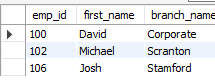
\includegraphics[width=0.4\textwidth]{./figs/JOINS.png}
        % 	\caption{\href{}{source}}
        \end{figure}
    
    \item Left joins:
        \begin{itemize}
            \item On a left join all of the table is included but only the one that matches.
        \end{itemize}
        \begin{minted}[autogobble]{sql}
            SELECT employee.emp_id, employee.first_name, branch.branch_name 
            FROM employee LEFT JOIN branch ON employee.emp_id = branch.mgr_id;
        \end{minted}
    
    \item Right join:
        \begin{minted}[autogobble]{sql}
            SELECT employee.emp_id, employee.first_name, branch.branch_name 
            FROM employee RIGHT JOIN branch ON employee.emp_id = branch.mgr_id;
        \end{minted}
    
    \item There is an outer join but this is not available in mysql.
\end{itemize}



% \chapter{Inheritance}
% \begin{itemize}
    \item Nested query is when you use multiple select statements within select statements to get specific information.
    \item Find names of all employees who have sold over 30,000 to a single client:
        \begin{minted}[autogobble]{sql}
            SELECT employee.first_name, employee.last_name, employee.emp_id
            FROM employee 
            WHERE employee.emp_id IN(
                    SELECT works_with.emp_id 
                    FROM works_with 
                    WHERE works_with.total_sales > 30000
            );
        \end{minted}
        \begin{figure}[H]
            \centering
            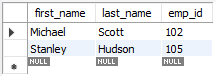
\includegraphics[width=0.4\textwidth]{./Figs/2020-12-24-21-51-11.png}
        % 	\caption{}
        \end{figure}
    
    \item Find all clients who are handled by the branch that Michael Scott manages, Assume you know Michael's ID.
        \begin{minted}[autogobble]{sql}
            SELECT client.client_name 
            FROM client 
            WHERE client.branch_id = (
                SELECT branch.branch_id 
                FROM branch 
                WHERE branch.mgr_id = 102
                LIMIT 1
            );
        \end{minted}
        \begin{figure}[H]
            \centering
            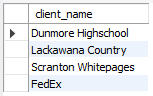
\includegraphics[width=0.4\textwidth]{./Figs/2020-12-24-21-51-49.png}
        % 	\caption{}
        \end{figure}
\end{itemize}


% \chapter{Polymorphism}
% \begin{itemize}
    \item How to delete entries when they have foreign keys linked to them.
    \item ON DELETE SET NULL is basically when we delete an employee all foreign associated to that employee is going to be set to null.
    \item ON CASCADE is basically when we delete an employee the rows in other tables containing employee ids pointing to the deleted employee are also going to get eliminated.
    \item The code below signifies that if the employee id in the employee table gets deleted the value of that foreign key is set to null. 
        \begin{minted}[autogobble]{sql}
            CREATE TABLE branch (
                branch_id INT PRIMARY KEY,
                branch_name VARCHAR(40),
                mgr_id INT,
                mgr_start_date DATE,
                FOREIGN KEY(mgr_id) REFERENCES employee(emp_id) ON DELETE SET NULL
            );
        \end{minted}
    
    \item You might want to consider using set null when the attribute being deleted is no essential, if it is essential then use cascade.
\end{itemize}


% \chapter{Smart pointers}
% \begin{itemize}
    \item A trigger is basically is a block of SQL code that will define what needs to happen when a certain operation gets performed on a database.
    
    \item Making a trigger needs to be done from the command line.
        \begin{minted}[autogobble]{sql}
            DELIMITER $$ 
                CREATE 
                    TRIGGER my_trigger BEFORE INSERT 
                    ON employee
                    FOR EACH ROW BEGIN 
                        INSERT INTO trigger_test VALUES('added new people');
                    END$$
                DELIMITER ;
        \end{minted}
    
    \item Example:
        \begin{minted}[autogobble]{sql}
            DELIMITERDELIMITER $$ 
                CREATE TRIGGER my_trigger2 BEFORE INSERT 
                ON employee 
                FOR EACH ROW BEGIN 
                    IF NEW.sex = 'M' THEN 
                        INSERT INTO trigger_test VALUES('added male employee');
                    ELSEIF NEW.sex = 'F' THEN 
                        INSERT INTO trigger_test VALUES('added female');
                    ELSE 
                        INSERT INTO trigger_test VALUES('added other employee');
                    END IF;
                END$$
            DELIMITER ;
        \end{minted}
    
    \item Use \mintinline{sql}{drop trigger} command to eliminate the trigger.
\end{itemize}


% \chapter{Exception handling}
% To design a database schema we must first understand it, for understanding we design ER programs, they stand for Entity Relationship Diagrams.
An ER diagram would be absolutely helpful in defining relationships so that we can understand the relations, object and attributes associated with each table in our database.
ER diagrams act as a middle man between the requirements and the actual schema that gets implemented.
\begin{itemize}
    \item ER diagrams consists of different shapes and symbols that establish relationships.
    \item An entity is an object we want to model and store information about. In ER diagrams they are modeled using a square or rectangle.
\end{itemize}

\begin{itemize}
    \item ER Diagrams: used to design the database, it is used to model an entity.
    \item An entity is depicted as a square, in this example the entities we want to model are students.
        \begin{figure}[H]
            \centering
            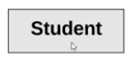
\includegraphics[width=0.4\textwidth]{./Figs/2020-12-23-23-33-10.png}
        % 	\caption{}
        \end{figure}
        
    \item An attribute is a specific piece of information about an entity. In ER diagrams they are modeled using ovals connected to entity.
        \begin{figure}[H]
            \centering
            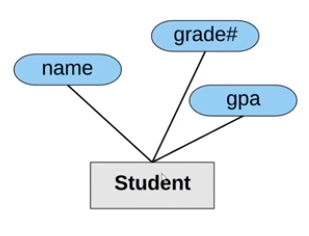
\includegraphics[width=0.4\textwidth]{./Figs/2020-12-23-23-33-26.png}
        % 	\caption{}
        \end{figure}
    \item Primary key: an attribute that uniquely identifies an entry in the database table. Modeled inside an oval, the primary key name is underlined.
        \begin{figure}[H]
            \centering
            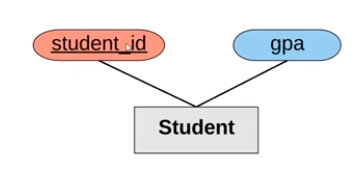
\includegraphics[width=0.4\textwidth]{./Figs/2020-12-23-23-33-54.png}
        % 	\caption{}
        \end{figure}
    \item Composite attributes: Attributes that can be broken up into sub-attributes. In this example the name attribute can be broken up further into first name and last name, this is a composite attribute.
        \begin{figure}[H]
            \centering
            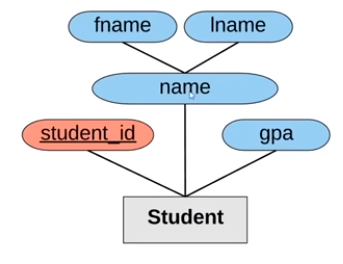
\includegraphics[width=0.4\textwidth]{./Figs/2020-12-23-23-34-47.png}
        % 	\caption{}
        \end{figure}
    \item Multi-valued attribute: an attribute that can have more than one value. Modeled with an oval with an inner oval. In this case ``clubs'' is a multi-values attribute because a student could be involved in more than one club or zero, it can have more than one value, they are not going to have more than one gpa or more than one name, but they can be involved in more than one club.
        \begin{figure}[H]
            \centering
            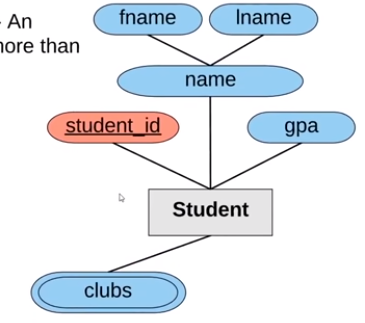
\includegraphics[width=0.4\textwidth]{./Figs/2020-12-23-23-35-38.png}
        % 	\caption{}
        \end{figure}
    \item Derived attribute: an attribute that can be derived from the other attributes, modeled using oval with dashed lines. A derived attribute is not stored in the database, they can be figured out whenever they are needed but for the sake of efficient memory usage they are not stored because they can be derived whenever they are needed. Has honors can be derived from the gpa.
        \begin{figure}[H]
            \centering
            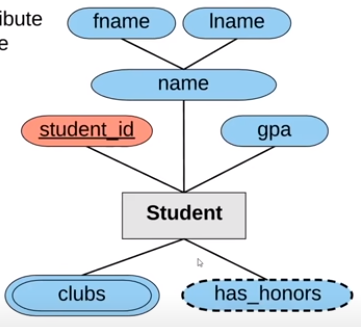
\includegraphics[width=0.4\textwidth]{./Figs/2020-12-23-23-37-32.png}
        % 	\caption{}
        \end{figure}
    \item Multiple entities: you can define more than one entity in the diagram. We can have multiple entities and establish relations between them, in this case lets define an entity called class. Notice the class entity has a primary key called class id.
        \begin{figure}[H]
            \centering
            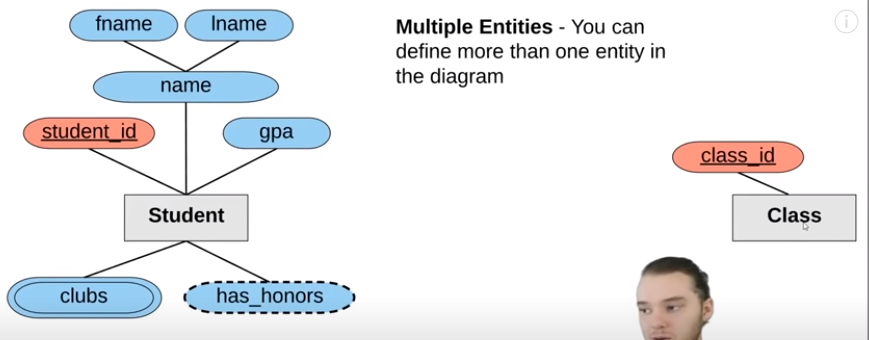
\includegraphics[width=0.4\textwidth]{./Figs/2020-12-23-23-40-02.png}
        % 	\caption{}
        \end{figure}
    \item Relationship: defines a relationship between two entities. Modeled using lines and a diamond shape. Using a double line means that task has total and one line means partial. When we have two or more entities we can define relationships between those two entities, here lets establish a relationship between student and class:
        \begin{itemize}
            \item A relationship is denoted by the diamond, in this case ``takes'', the lines connecting the entities to the relationship also hold particular information. 
            \item The relationship here is that a student can take a class and a class can be taken by a student.
            \item In many ways relationships are denoted as verbs, and they can go both ways, in this case you can say the student takes a class and the class takes a student.
            \item One line means partial participation, meaning that not all students need to take a class.
            \item Two lines means total participation, meaning that all the classes need to be taken by at least a minimum of students, it doesn't make sense to have a class that has zero students taking it.
        \end{itemize}
        \begin{figure}[H]
            \centering
            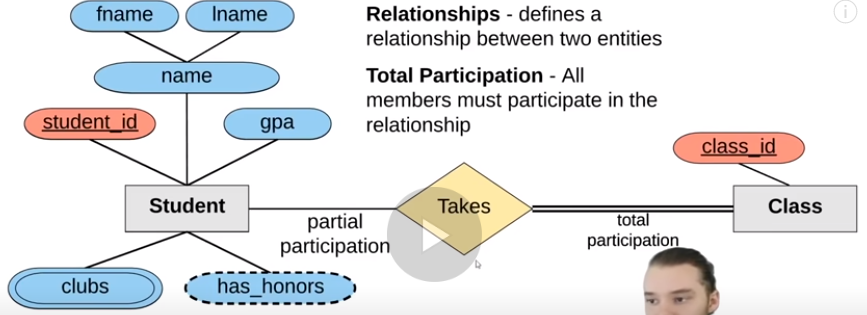
\includegraphics[width=0.4\textwidth]{./Figs/2020-12-23-23-41-52.png}
        % 	\caption{}
        \end{figure}
    \item Relationship attribute: an attribute about the relationship. In this case there is an attribute on the relationship, the entity student takes a class, while he takes the class the entity student will receive a grade, this only happens when the student takes the class. It doesn't make sense to store in student grades on classes he never took or never will.
        \begin{figure}[H]
            \centering
            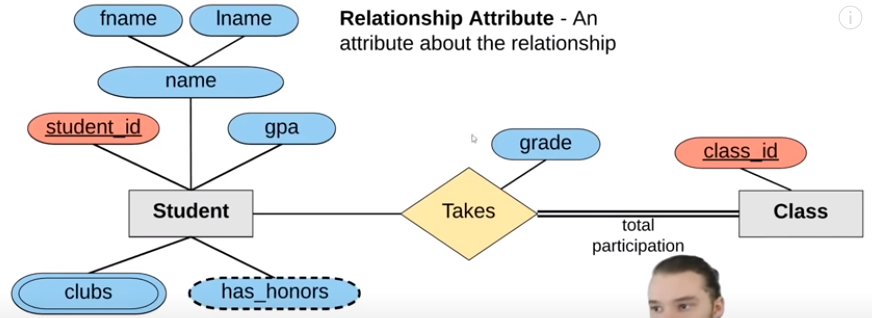
\includegraphics[width=0.4\textwidth]{./Figs/2020-12-23-23-47-13.png}
        % 	\caption{}
        \end{figure}
    \item Relationship cardinality: the number of instances of an entity from a relation that can associated with the relation. This means for our example that a student can take multiple classes, and we can define the same thing for the class, we can say the class is taken by any number of students. However, we can define cardinality relationships as the following:
        \begin{itemize}
            \item 1:1, meaning that a student can take one class and a class can be taken one student. This means that the class can only have one student and the student can only take one class. Doesn't make very much sense in this example.
            \item 1:N, N meaning a constant number of students, 1:N means that a student can take one class and a class can be taken by N number of students.
            \item N:M, means that a student can take any number of classes and a class can be taken by any number of students.
            \item This is relevant because it is useful in data modeling requirements, for example if you require your database to check that a student can only take one class at a time, then that is something you want to consider in your ER diagrams.
        \end{itemize}
        \begin{figure}[H]
            \centering
            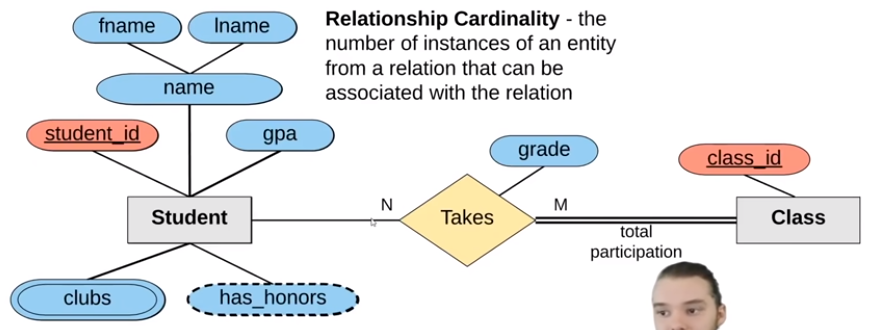
\includegraphics[width=0.4\textwidth]{./Figs/2020-12-23-23-52-17.png}
        % 	\caption{}
        \end{figure}
    \item Weak entity: an entity that cannot be uniquely identified by its attributes alone, an entity that will depend on another.
        \begin{itemize}
            \item In this example a weak entity is an exam, notice that a class can have an exam, the exam is an entity, the exam has the primary key of exam id, but in this case an exam can't exist without a class, in order for an exam to exist it has to be associated with a class.
        \end{itemize}
        \begin{figure}[H]
            \centering
            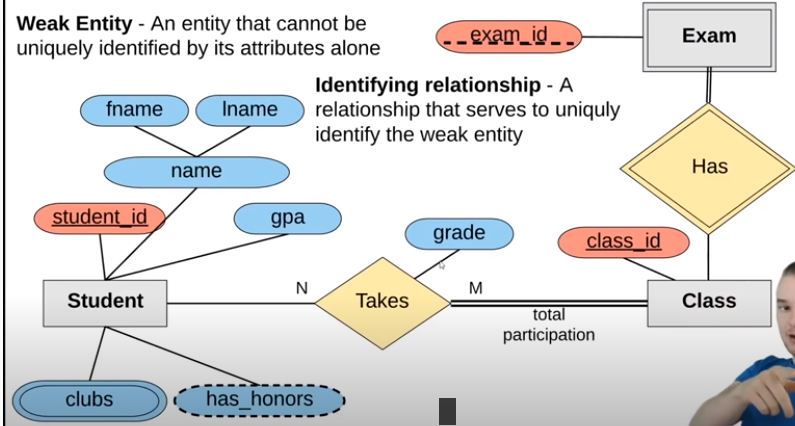
\includegraphics[width=0.4\textwidth]{./Figs/2020-12-23-23-53-53.png}
        % 	\caption{}
        \end{figure}
    \item Identifying relationship: a relationship that serves to uniquely identify the weak entity.
        \begin{itemize}
            \item In this example the identifying relationship is the ``has'', an exam can be uniquely \emph{identified} only if there is a class associated with it. 
            \item The exam does not exist on its own, it relies on a class for an identity.
            \item Whenever we have a weak entity and identifying relationship the weak entity always has to have total participation in the identifying relationship, all exams must have a class but not all classes need to have an exam.
        \end{itemize}
        \begin{figure}[H]
            \centering
            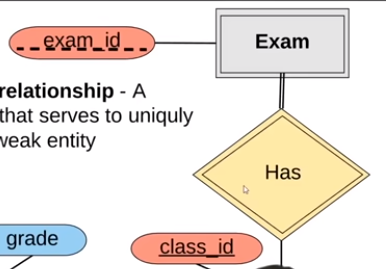
\includegraphics[width=0.4\textwidth]{./Figs/2020-12-23-23-55-58.png}
        % 	\caption{}
        \end{figure}
\end{itemize}

Knowing this, we can take this ER diagram and convert it to a actual database schema.


% \chapter{I/O and streams}
% Using a Data Requirements document we can construct an ER diagram, take for example the following:
\begin{verbatim}
    Company Data Requirements:
    The company is organized into branches. Each branch has a unique number, a name, and a particular employee who manages it.

    The company makes it's money by selling to clients. Each client has a name and unique number to identify it.

    The foundation of the company is it's employees. Each employee has a name, birthday, sex, salary and unique number to identify it.

    An employee can work for one branch at a time, and each branch will be managed by one of the employees that work there. We'll also want to keep track of when the current manager started as manager.

    An employee can act as a supervisor for other employees at the branch, an employee may also act as the supervisor for employees at other branches. An employee can have at most one supervisor.

    A branch may handle a number of clients, with each client having a name and a unique number to identify it. A single client may only be handled by one branch at a time.

    Employees can work with clients controlled by their branch to sell them stuff. If necesary, multiple employees can work with the same client. We'll want oto keep track of how many dollars worth of stuff each employee sells to each client they work with.

    Many branches will need to work with suppliers to buy inventory. For each supplier we'll keep track of their name and the type of product they're selling the branch. A single suppler may supply products to multiple branches.
\end{verbatim}

\section{Conversion of the Data Requirements Document into an ER diagram}
Each sentence conveys critical information, lets look at it one at a time and see how the ER diagram turns out:
\begin{itemize}
    \item \textbf{The company is organized into branches. Each branch has a unique number, a name, and a particular employee who manages it.}
        \begin{figure}[H]
            \centering
            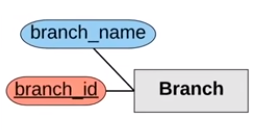
\includegraphics[width=0.4\textwidth]{./Figs/2020-12-24-00-13-51.png}
        % 	\caption{}
        \end{figure}
    
    \item \textbf{The company makes it's money by selling to clients. Each client has a name and unique number to identify it.}
        \begin{figure}[H]
            \centering
            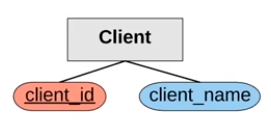
\includegraphics[width=0.4\textwidth]{./Figs/2020-12-24-00-14-18.png}
        % 	\caption{}
        \end{figure}
    
    \item \textbf{The foundation of the company is it's employees. Each employee has a name, birthday, sex, salary and unique number to identify it.}
        \begin{figure}[H]
            \centering
            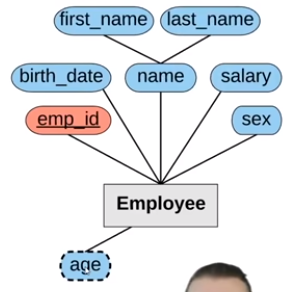
\includegraphics[width=0.4\textwidth]{./Figs/2020-12-24-00-14-53.png}
        % 	\caption{}
        \end{figure}
    
    \item \textbf{An employee can act as a supervisor for other employees at the branch, an employee may also act as the supervisor for employees at other branches. An employee can have at most one supervisor.}
        \begin{itemize}
            \item Notice here the data is defining a relationship.
            \item The relationship is the ``work for''.
            \item All branches must have employees working for them, and all employees must work for a branch. This means a both way total participation.
            \item An employee can work only for ONE branch, and a branch can have multiple employees, hence this is a 1:N cardinality relationship.
        \end{itemize}
        \begin{figure}[H]
            \centering
            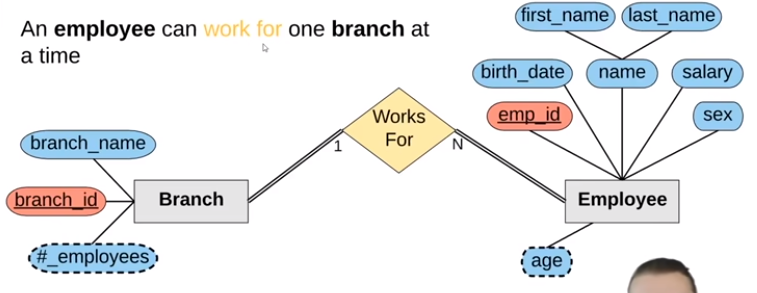
\includegraphics[width=0.4\textwidth]{./Figs/2020-12-24-00-16-07.png}
        % 	\caption{}
        \end{figure}
    
    \item \textbf{An employee can work for one branch at a time, and each branch will be managed by one of the employees that work there. We'll also want to keep track of when the current manager started as manager.}
        \begin{itemize}
            \item Notice the cardinality relationship here, a branch can be managed by one employee and an employee can manage one branch, its 1:1. 
            \item On the ``manages'' relationship we must store the attribute start date, this records when the manager started as manager.
        \end{itemize}
        \begin{figure}[H]
            \centering
            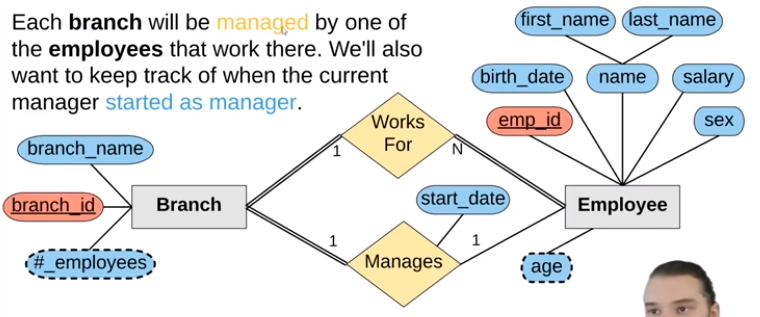
\includegraphics[width=0.4\textwidth]{./Figs/2020-12-24-00-20-01.png}
        % 	\caption{}
        \end{figure}
    
    \item \textbf{An employee can act as a supervisor for other employees at the branch, an employee may also act as the supervisor for employees at other branches. An employee can have at most one supervisor.}
        \begin{itemize}
            \item Here notice that we have a relationship that is with one's self, meaning that an employee can act as a supervisor to other employees, but the supervisor is himself an employee as well.
            \item Lets call the supervisor relationship the ``supervision'' relationship, notice that it is comprised with a supervisor and the supervisee, an employee can have at most one supervisor, and a supervisor can have multiple people to supervise, all the while being an employee also.
            \item The cardinality relationship is thus a 1:N relationship. Because an employee can have at most one supervisor but a supervisor can supervise several employees.
        \end{itemize}
        \begin{figure}[H]
            \centering
            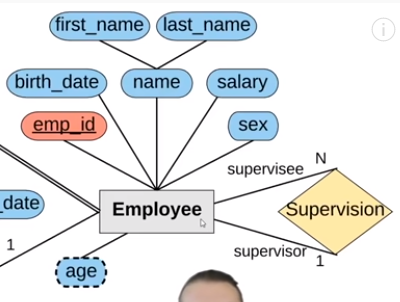
\includegraphics[width=0.4\textwidth]{./Figs/2020-12-24-00-32-14.png}
        % 	\caption{}
        \end{figure}
    
    \item \textbf{A branch may handle a number of clients, with each client having a name and a unique number to identify it. A single client may only be handled by one branch at a time.}
        \begin{itemize}
            \item Now notice the relationship happening between the branch and the client, the client can be handled any number of times by a branch and a single client can only be handled by one branch at a time.
            \item Notice the cardinality relationship, the branch can handle any number of clients but the client can only be handled by only one branch at a time.
            \item Notice that the client has a total participation, because every client needs to be handled by a branch, but the branch has a partial participation because not all branches need to handle every client, in this case it needs to be one branch at a time.
        \end{itemize}
        \begin{figure}[H]
            \centering
            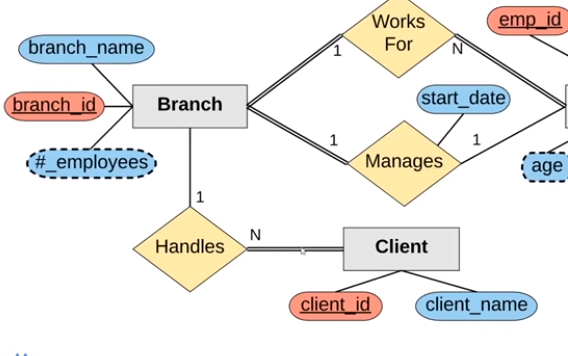
\includegraphics[width=0.4\textwidth]{./Figs/2020-12-24-00-38-06.png}
        % 	\caption{}
        \end{figure}
    
    \item \textbf{Employees can work with clients controlled by their branch to sell them stuff. If necesary, multiple employees can work with the same client. We'll want oto keep track of how many dollars worth of stuff each employee sells to each client they work with.}
        \begin{itemize}
            \item Notice the cardinality, employees can work with clients, any number of clients and clients can have any number of employees working with them, It's an N:M cardinality relationship.
            \item Notice here the relationship is the client and the employee ``working'' together, or ``works with''. When this relationship takes place a sale may take place, this is a relationship attribute ``sales''.
            \item Notice the participation, all clients must work with and interact with employees but not all employees must work with clients.
        \end{itemize}
        \begin{figure}[H]
            \centering
            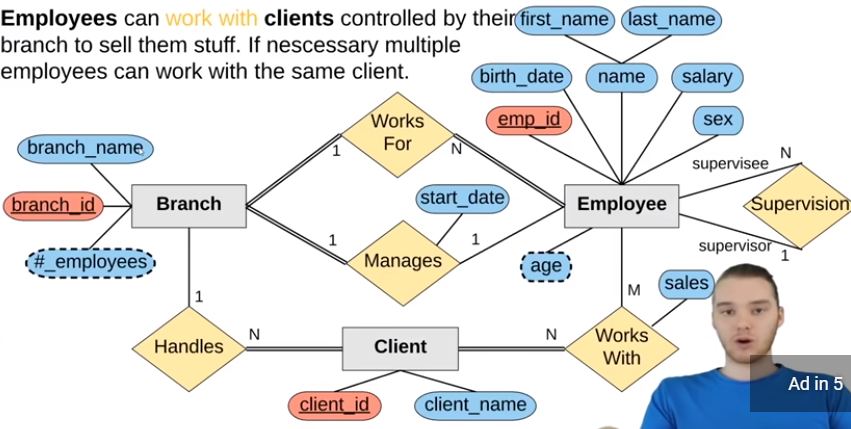
\includegraphics[width=0.4\textwidth]{./Figs/2020-12-24-00-39-58.png}
        % 	\caption{}
        \end{figure}

    \item \textbf{Many branches will need to work with suppliers to buy inventory. For each supplier we'll keep track of their name and the type of product they're selling the branch. A single suppler may supply products to multiple branches.}
        \begin{itemize}
            \item This is a case where we would need to define a weak entity and weak relationship.
            \item Notice the branch supplier supplies a specific branch or branches, we also want to keep track of which supplier is supplying with branch. Do this using the weak relationship ``supplies''.
            \item Notice that there can be any number of suppliers per branch and any branches per supplier. The cardinality relationship is N:M.
            \item Notice the participation, as always weak entities have total participation in the relationship and the string entity haves in this case partial participation, because not all branches must be supplied. 
        \end{itemize}
        \begin{figure}[H]
            \centering
            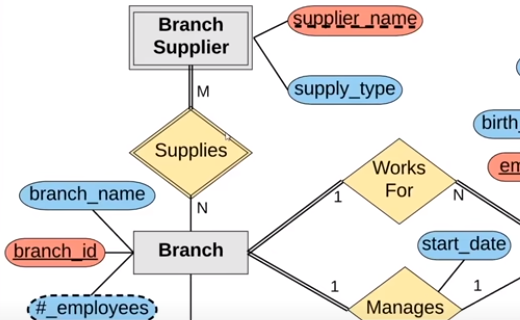
\includegraphics[width=0.4\textwidth]{./Figs/2020-12-24-00-48-35.png}
        % 	\caption{}
        \end{figure}
    
    \item The whole diagram looks like this:
        \begin{figure}[H]
            \centering
            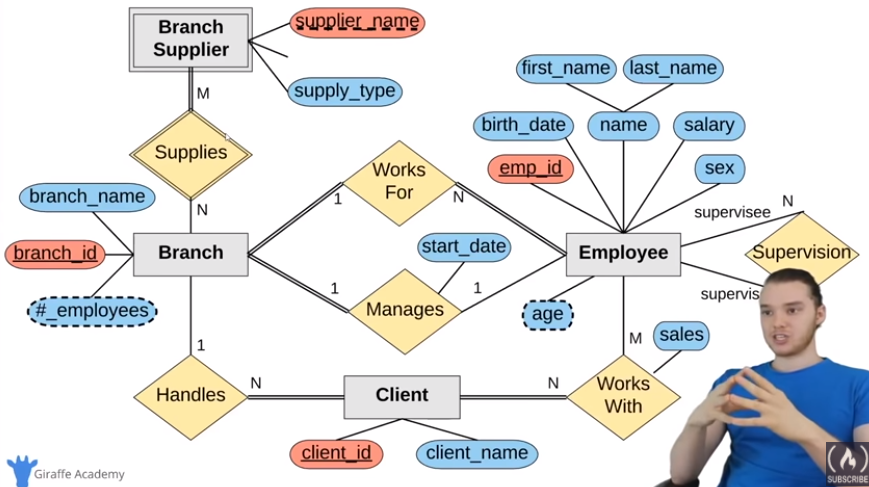
\includegraphics[width=0.4\textwidth]{./Figs/2020-12-24-00-50-11.png}
        % 	\caption{}
        \end{figure}
\end{itemize}



% \chapter{The standard template library (STL)}
% Converting the following into a schema:
\begin{figure}[H]
    \centering
    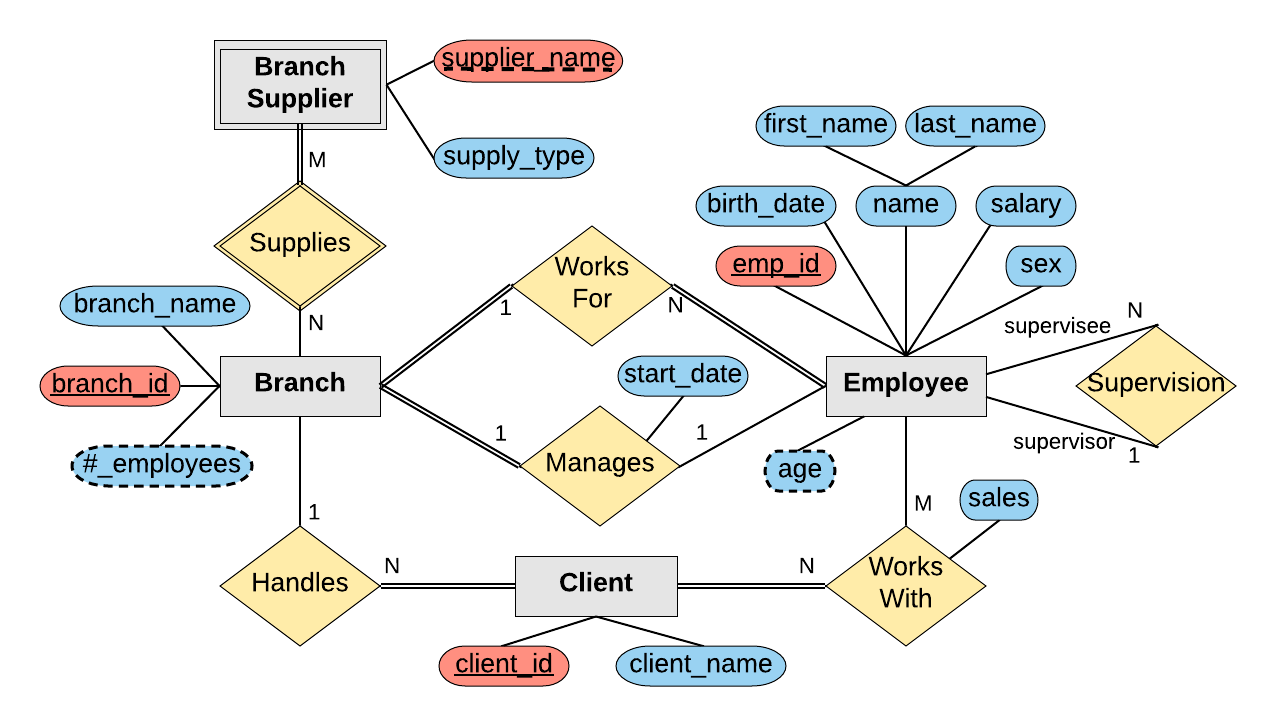
\includegraphics[width=0.8\textwidth]{./Figs/2020-12-24-22-51-10.png}
% 	\caption{}
\end{figure}

\section{Steps}
\begin{enumerate}
    \item Mapping of regular entity types:
        \begin{figure}[H]
            \centering
            \includegraphics[width=0.4\textwidth]{./Figs/2020-12-24-22-59-55.png}
        % 	\caption{}
        \end{figure}
        \begin{itemize}
            \item For each regular entity type create a relation or table that includes all the simple attributes of that entity.
            \item In this case the regular entities are Branch, Employee, and Client. The columns of the table of the entities will be the simple attributes of the entities.
            \item Notice we don't mark the relationships between the entities nor the branch supplier as an entity because in this case the branch supplier is a weak entity.
            \item In composite attribute it is common to store the attributes that compose the composite attribute rather than storing it as a composite attribute. This means that for example name is composed of first name and last name, but we will not store it as name but rather as first and last name directly. Composite attributes are stored as subattributes.
        \end{itemize}
        \begin{figure}[H]
            \centering
            \includegraphics[width=0.4\textwidth]{./Figs/2020-12-24-22-58-24.png}
        % 	\caption{}
        \end{figure}
        
    \item Mapping of weak entity types:
        \begin{figure}[H]
            \centering
            \includegraphics[width=0.4\textwidth]{./Figs/2020-12-24-23-00-07.png}
        % 	\caption{}
        \end{figure}
        \begin{itemize}
            \item For each weak entity type create a relation (table) that includes all simple attributes of the weak entity.
            \item The primary key of the weak entity of the new table should be the partial key of the weak entity plus the primary key of its owner. In this case the primary key will be branch id.
        \end{itemize}
        \begin{figure}[H]
            \centering
            \includegraphics[width=0.4\textwidth]{./Figs/2020-12-24-22-57-54.png}
        % 	\caption{}
        \end{figure}
    
    \item Mapping of Binary 1:1 relationship types:
        \begin{figure}[H]
            \centering
            \includegraphics[width=0.4\textwidth]{./Figs/2020-12-24-23-00-49.png}
        % 	\caption{}
        \end{figure}
        \begin{itemize}
            \item For each one to one binary relationship we want to include one side of the relationship as a foreign key in the other favor total participation.
            \item Basically include the primary key of one of these entities as a foreign key in the other's entity relation. And if a particular entity has total participation in the relationship then you want to add the foreign key on to the one that has total participation, in this case to branch, add the employee primary key as a foreign key to branch.
            \item If both of them are total participation or both are partial participation then it is left to your discretion to decide which entity has the foreign key.
            \item To the table Branch, add the foreign key of employee, in this case called mgr\_id will be foreign key to link the relationship.
        \end{itemize}
        \begin{figure}[H]
            \centering
            \includegraphics[width=0.4\textwidth]{./Figs/2020-12-24-23-05-49.png}
        % 	\caption{}
        \end{figure}
    
    \item Mapping of binary 1:N relationship types:
        \begin{figure}[H]
            \centering
            \includegraphics[width=0.4\textwidth]{./Figs/2020-12-24-23-07-54.png}
        % 	\caption{}
        \end{figure}
        \begin{itemize}
            \item Include the 1 side's primary key as a foreign key in the N side relation table.
            \item In this case we have three.
            \item Basically, in the case where we establish the relationship between the branch works for employee, I want to include the 1's side primary key, which means the branch side, as a foreign key in the employee table, this means that employee will have a column as a foreign key specifying the branch.
            \item In the employee supervision relation, we grab the 1's side, which is employee and store in the N's side, which is employee, the foreign key to the supervisor.
            \item In the branch handles client relationship we store as a foreign key a branch in client.
        \end{itemize}
    
    \item Mapping of binary M:N relationship types:
        \begin{figure}[H]
            \centering
            \includegraphics[width=0.4\textwidth]{./Figs/2020-12-24-23-16-49.png}
        % 	\caption{}
        \end{figure}
        \begin{itemize}
            \item Create a new table who's primary key is a combination of both entities' primary key's. Also include any relationship attributes.
            \item In this case store sales.
        \end{itemize}
        \begin{figure}[H]
            \centering
            \includegraphics[width=0.4\textwidth]{./Figs/2020-12-24-23-16-39.png}
        % 	\caption{}
        \end{figure}
\end{enumerate}
You should end up with the tables looking like this:
\begin{figure}[H]
    \centering
    \includegraphics[width=0.4\textwidth]{./Figs/2020-12-24-23-32-40.png}
    \includegraphics[width=0.4\textwidth]{./Figs/2020-12-24-23-14-01.png}
    \includegraphics[width=0.4\textwidth]{./Figs/2020-12-24-23-14-09.png}
    \includegraphics[width=0.4\textwidth]{./Figs/2020-12-24-23-14-17.png}
    \includegraphics[width=0.4\textwidth]{./Figs/2020-12-24-23-33-07.png}
% 	\caption{}
\end{figure}
You can see the relationships like this:
\begin{figure}[H]
    \centering
    \includegraphics[width=0.4\textwidth]{./Figs/2020-12-24-23-34-55.png}
% 	\caption{}
\end{figure}

Now we can populate the database in the way weve already learned.
\begin{figure}[H]
    \centering
    \includegraphics[width=0.8\textwidth]{./Classes/company-database.pdf}
% 	\caption{}
\end{figure}



%%%%%%%%%%%%%%%%%%%%%%%%%%%%%%%%%%%%%%%%%%%%%%%%%%%%%%%%%%%%%%%%%%%%%%%%%%%%%%%%%%%%%%%%%%%%%%%%%%%%%%%%%%%%%%%%%%%%%%%%%%%%%%%%%%%%%%%%%%%%%%
\end{document}

